\documentclass[11pt,a4paper]{article}
\usepackage {amsmath,amsthm}
\usepackage{geometry}
\usepackage{titlesec}
\geometry{a4paper}
\usepackage{natbib}
\usepackage{caption}
\captionsetup{skip=0pt}
\usepackage{multirow}
%\bibliographystyle{econ}


\usepackage [pdftex]{graphicx}

\usepackage[hidelinks]{hyperref}
%\usepackage[colorlinks=true, urlcolor=blue, pdfborder={0 0 0}]{hyperref}
%\usepackage{comment}
\usepackage{sectsty}
\sectionfont{\fontsize{14}{15}\selectfont}
\subsectionfont{\fontsize{13}{15}\selectfont}

\titleformat*{\section}{\LARGE\bfseries}
\titleformat*{\subsection}{\Large\bfseries}
\usepackage{booktabs}
\usepackage{float}
\usepackage{makecell}
\usepackage{subcaption}
\usepackage{setspace}
\usepackage{placeins}
\usepackage{dcolumn}
\usepackage{float}
\newtheorem{theorem}{Proposition}

\title{\Large Crying Wolf in the Lab\\}
\author{\large Arya Gaduh, Peter McGee, Alexander Ugarov*}
\begin{document}
\maketitle
\onehalfspacing
\begin{abstract}{ }


\vspace{10pt}
\begin{singlespace}

\noindent {\footnotesize{}Keywords: }{\thispagestyle{empty}}
\end{singlespace}
\end{abstract}

\vspace{140pt}
\footnotesize






\onehalfspacing
\normalsize
\newpage
\section{Introduction}

\appendix


\section{Results}

\subsection{IP and Beliefs}
\begin{figure}[H]
\centering
\caption{Average Blind Protection Response} \label{Blind Protection Responses}

  \centering
  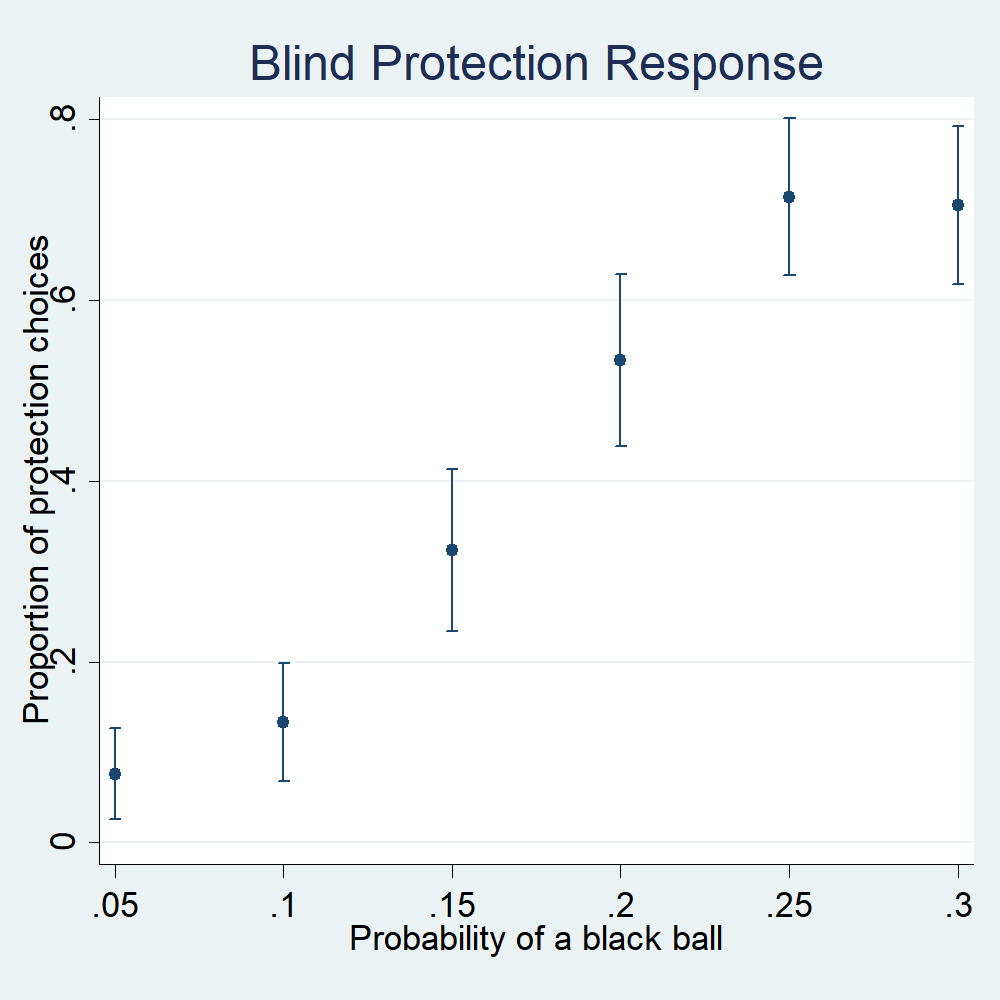
\includegraphics[scale=0.3]{Graphs/blind_prot_sta.png}

\end{figure}

\begin{figure}[H]
\centering
\caption{Average Informed Protection Response} \label{Informed Protection Responses}

  \centering
  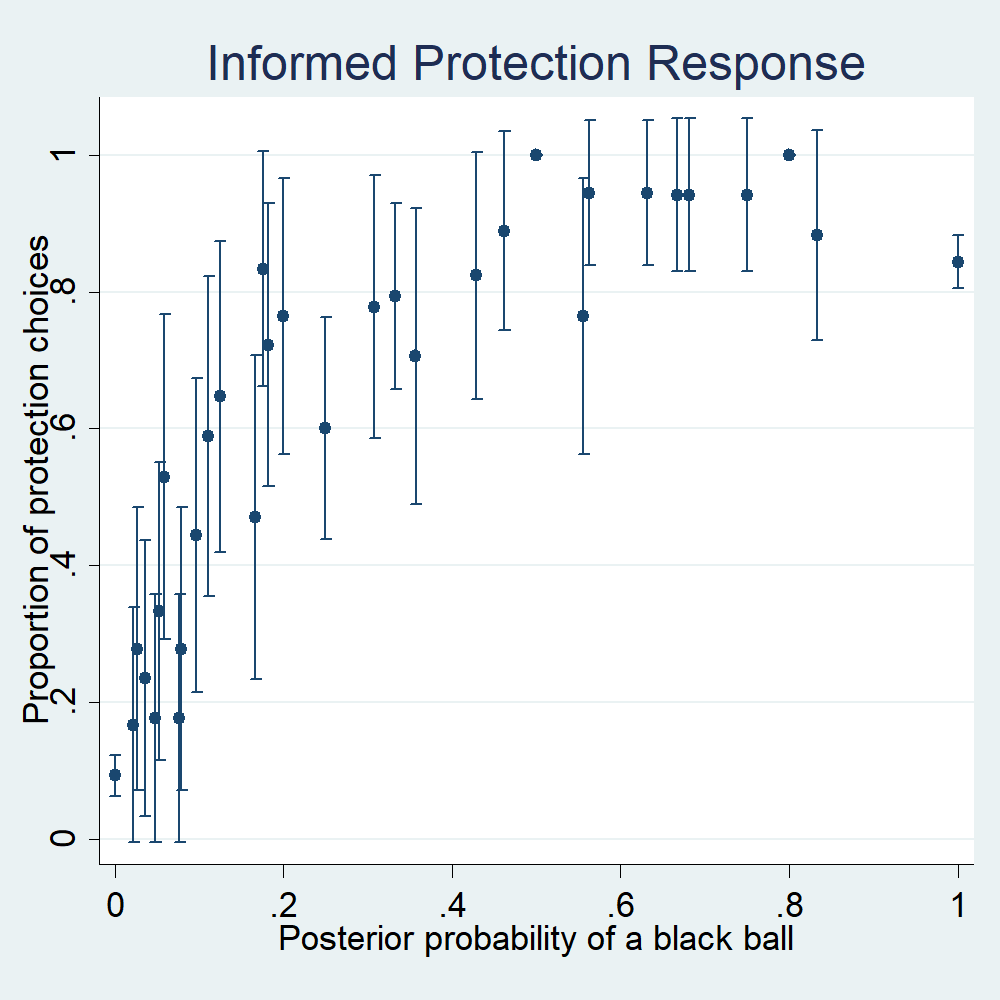
\includegraphics[scale=0.3]{Graphs/ip_response.png}

\end{figure}


\clearpage
(1)&No&No  &White&0.000&0.067&0.000&0.000\\
(2)&No&Yes &White&0.100&0.333&0.000&0.000\\
(3)&Yes&No &White&0.000&0.130&0.000&0.000\\
(4)&Yes&Yes&White&0.131&0.564&0.121&0.000\\
(5)&No&No  &Black&1.000&0.846&1.000&0.000\\
(6)&No&Yes &Black&1.000&0.841&1.000&0.000\\
(7)&Yes&No &Black&0.550&0.833&0.870&0.355\\
(8)&Yes&Yes&Black&0.483&0.886&0.871&0.685\\

1&No&No&White&0.000&0.039&0.001\\
2&No&Yes&White&0.045&0.140&0.000\\
3&Yes&No&White&0.000&0.116&0.000\\
4&Yes&Yes&White&0.062&0.245&0.000\\
5&No&No&Black&1.000&-0.187&0.000\\
6&No&Yes&Black&1.000&-0.332&0.000\\
7&Yes&No&Black&0.396&0.177&0.000\\
8&Yes&Yes&Black&0.328&0.192&0.000\\

ALEX: Double check: Are these everyone or p $\leq$ 0.2?
YES


\newpage
FP rate x (S=White)&     .676\sym{***}&     .552\sym{**} &     .379\sym{*}  &     .309         \\
                &    (3.5)         &    (2.2)         &    (1.9)         &    (1.2)         \\
FN rate x (S=White)&     1.08\sym{**} &     1.57\sym{***}&     .583         &     1.04\sym{**} \\
                &    (2.3)         &    (3.3)         &    (1.2)         &    (2.1)         \\
S=Black         &      1.2\sym{**} &     2.13\sym{***}&     .706         &     1.56\sym{***}\\
                &    (2.1)         &    (3.8)         &    (1.3)         &    (2.7)         \\
FP rate x (S=Black)&    -.887         &    -1.57\sym{*}  &    -.507         &    -1.05         \\
                &   (-1.0)         &   (-1.9)         &   (-0.6)         &   (-1.4)         \\
FN rate x (S=Black)&   -.0383         &    -.372\sym{*}  &   -.0542         &    -.372\sym{*}  \\
                &   (-0.3)         &   (-1.9)         &   (-0.3)         &   (-1.7)         \\
p$=$0.2         &     .404\sym{***}&     .363\sym{***}&     .357\sym{***}&     .316\sym{***}\\
                &    (9.5)         &    (7.1)         &    (7.1)         &    (5.0)         \\
FP rate x (p=0.2)&                  &      .55\sym{*}  &                  &     .405         \\
                &                  &    (1.7)         &                  &    (1.2)         \\
FN rate x (p=0.2)&                  &     .518\sym{*}  &                  &      .52\sym{*}  \\
                &                  &    (1.8)         &                  &    (1.8)         \\
\hline
N               &      582         &      582         &      582         &      582         \\
Pseudo R-squared&     .575         &     .585         &     .609         &     .617         \\
Log-likelihood  &     -172         &     -168         &     -158         &     -154         \\


ALEX: 
\begin{itemize}
	\item IP Table: 
		\begin{itemize}
			\item We have Table 23 (new version) that controls for beliefs -> finds that beliefs explain biases except for s=white, FP.
			\item We want to tell the story of what happens (or the biases that remain) once we account for belief errors.
		\end{itemize}
	%\item Add table where we only have p=0.1,0.2; p=0.3, 0.5
\end{itemize}

\newpage

\begin{table}[htbp]\centering
\def\sym#1{\ifmmode^{#1}\else\(^{#1}\)\fi}
\caption{Belief Elicitation: When Mistakes Happen}
\begin{tabular}{l*{3}{c}}
\hline\hline
                &\multicolumn{1}{c}{(1)}&\multicolumn{1}{c}{(2)}&\multicolumn{1}{c}{(3)}\\
                &\multicolumn{1}{c}{All}&\multicolumn{1}{c}{S=White}&\multicolumn{1}{c}{S=Black}\\
\hline
FP rate         &    0.600\sym{***}&    0.292\sym{***}&    0.908\sym{***}\\
                &  (0.057)         &  (0.063)         &  (0.102)         \\
FN rate         &    0.011         &    0.273\sym{***}&   -0.251\sym{***}\\
                &  (0.053)         &  (0.061)         &  (0.084)         \\
A92             &   -0.018\sym{*}  &   -0.145\sym{***}&    0.108\sym{***}\\
                &  (0.009)         &  (0.010)         &  (0.016)         \\
B113            &   -0.088\sym{***}&   -0.372\sym{***}&    0.196\sym{***}\\
                &  (0.009)         &  (0.010)         &  (0.016)         \\
B139            &    0.140\sym{***}&   -0.190\sym{***}&    0.470\sym{***}\\
                &  (0.000)         &  (0.000)         &  (0.000)         \\
B61             &   -0.170\sym{***}&   -0.177\sym{***}&   -0.163\sym{***}\\
                &  (0.000)         &  (0.000)         &  (0.000)         \\
B87             &    0.084\sym{***}&   -0.305\sym{***}&    0.473\sym{***}\\
                &  (0.001)         &  (0.001)         &  (0.002)         \\
C108            &    0.104\sym{***}&   -0.299\sym{***}&    0.506\sym{***}\\
                &  (0.001)         &  (0.001)         &  (0.002)         \\
C134            &    0.006         &   -0.205\sym{***}&    0.217\sym{***}\\
                &  (0.009)         &  (0.010)         &  (0.016)         \\
C56             &    0.005         &   -0.326\sym{***}&    0.337\sym{***}\\
                &  (0.009)         &  (0.010)         &  (0.016)         \\
C82             &    0.056\sym{***}&   -0.248\sym{***}&    0.360\sym{***}\\
                &  (0.000)         &  (0.000)         &  (0.000)         \\
D103            &    0.123\sym{***}&   -0.207\sym{***}&    0.453\sym{***}\\
                &  (0.000)         &  (0.000)         &  (0.000)         \\
D129            &    0.086\sym{***}&   -0.326\sym{***}&    0.498\sym{***}\\
                &  (0.001)         &  (0.001)         &  (0.002)         \\
D51             &    0.070\sym{***}&   -0.241\sym{***}&    0.381\sym{***}\\
                &  (0.001)         &  (0.001)         &  (0.002)         \\
D77             &    0.024\sym{**} &   -0.289\sym{***}&    0.337\sym{***}\\
                &  (0.009)         &  (0.010)         &  (0.016)         \\
E124            &    0.084\sym{***}&   -0.350\sym{***}&    0.518\sym{***}\\
                &  (0.000)         &  (0.000)         &  (0.000)         \\
E150            &    0.125\sym{***}&   -0.312\sym{***}&    0.561\sym{***}\\
                &  (0.001)         &  (0.001)         &  (0.002)         \\
E46             &    0.052\sym{***}&   -0.340\sym{***}&    0.443\sym{***}\\
                &  (0.000)         &  (0.000)         &  (0.000)         \\
E72             &    0.071\sym{***}&   -0.265\sym{***}&    0.406\sym{***}\\
                &  (0.001)         &  (0.001)         &  (0.002)         \\
E98             &    0.142\sym{***}&   -0.116\sym{***}&    0.400\sym{***}\\
                &  (0.009)         &  (0.010)         &  (0.016)         \\
F119            &    0.003         &   -0.314\sym{***}&    0.319\sym{***}\\
                &  (0.009)         &  (0.010)         &  (0.016)         \\
F41             &    0.080\sym{***}&   -0.307\sym{***}&    0.467\sym{***}\\
                &  (0.009)         &  (0.010)         &  (0.016)         \\
F67             &    0.123\sym{***}&   -0.334\sym{***}&    0.580\sym{***}\\
                &  (0.000)         &  (0.000)         &  (0.000)         \\
F93             &    0.093\sym{***}&   -0.305\sym{***}&    0.490\sym{***}\\
                &  (0.001)         &  (0.001)         &  (0.002)         \\
G114            &    0.122\sym{***}&   -0.284\sym{***}&    0.528\sym{***}\\
                &  (0.001)         &  (0.001)         &  (0.002)         \\
G140            &   -0.023\sym{**} &   -0.065\sym{***}&    0.018         \\
                &  (0.009)         &  (0.010)         &  (0.016)         \\
G62             &   -0.002         &   -0.425\sym{***}&    0.420\sym{***}\\
                &  (0.009)         &  (0.010)         &  (0.016)         \\
G88             &    0.039\sym{***}&   -0.315\sym{***}&    0.393\sym{***}\\
                &  (0.000)         &  (0.000)         &  (0.000)         \\
H109            &    0.122\sym{***}&   -0.287\sym{***}&    0.532\sym{***}\\
                &  (0.000)         &  (0.000)         &  (0.000)         \\
H135            &    0.070\sym{***}&   -0.341\sym{***}&    0.481\sym{***}\\
                &  (0.001)         &  (0.001)         &  (0.002)         \\
H57             &   -0.022\sym{***}&   -0.301\sym{***}&    0.256\sym{***}\\
                &  (0.001)         &  (0.001)         &  (0.002)         \\
H83             &    0.082\sym{***}&   -0.280\sym{***}&    0.444\sym{***}\\
                &  (0.009)         &  (0.010)         &  (0.016)         \\
I104            &   -0.003         &   -0.193\sym{***}&    0.187\sym{***}\\
                &  (0.009)         &  (0.010)         &  (0.016)         \\
I130            &    0.090\sym{***}&   -0.247\sym{***}&    0.427\sym{***}\\
                &  (0.000)         &  (0.000)         &  (0.000)         \\
I52             &    0.010\sym{***}&   -0.215\sym{***}&    0.235\sym{***}\\
                &  (0.000)         &  (0.000)         &  (0.000)         \\
I78             &    0.127\sym{***}&   -0.277\sym{***}&    0.531\sym{***}\\
                &  (0.001)         &  (0.001)         &  (0.002)         \\
J125            &    0.037\sym{***}&   -0.047\sym{***}&    0.121\sym{***}\\
                &  (0.009)         &  (0.010)         &  (0.016)         \\
J151            &   -0.043\sym{***}&   -0.157\sym{***}&    0.070\sym{***}\\
                &  (0.000)         &  (0.000)         &  (0.000)         \\
J47             &    0.073\sym{***}&   -0.264\sym{***}&    0.409\sym{***}\\
                &  (0.009)         &  (0.010)         &  (0.016)         \\
J73             &    0.162\sym{***}&   -0.212\sym{***}&    0.537\sym{***}\\
                &  (0.000)         &  (0.000)         &  (0.000)         \\
J99             &    0.041\sym{***}&   -0.235\sym{***}&    0.316\sym{***}\\
                &  (0.001)         &  (0.001)         &  (0.002)         \\
K120            &    0.127\sym{***}&   -0.277\sym{***}&    0.531\sym{***}\\
                &  (0.001)         &  (0.001)         &  (0.002)         \\
K42             &    0.004\sym{***}&   -0.324\sym{***}&    0.331\sym{***}\\
                &  (0.001)         &  (0.001)         &  (0.002)         \\
K68             &    0.035\sym{***}&   -0.213\sym{***}&    0.283\sym{***}\\
                &  (0.009)         &  (0.010)         &  (0.016)         \\
K94             &    0.056\sym{***}&   -0.298\sym{***}&    0.410\sym{***}\\
                &  (0.000)         &  (0.000)         &  (0.000)         \\
L115            &    0.081\sym{***}&   -0.152\sym{***}&    0.313\sym{***}\\
                &  (0.000)         &  (0.000)         &  (0.000)         \\
L141            &   -0.056\sym{***}&   -0.201\sym{***}&    0.090\sym{***}\\
                &  (0.001)         &  (0.001)         &  (0.002)         \\
L63             &    0.056\sym{***}&   -0.320\sym{***}&    0.431\sym{***}\\
                &  (0.001)         &  (0.001)         &  (0.002)         \\
L89             &    0.089\sym{***}&   -0.135\sym{***}&    0.314\sym{***}\\
                &  (0.009)         &  (0.010)         &  (0.016)         \\
M110            &    0.008         &   -0.033\sym{***}&    0.048\sym{***}\\
                &  (0.009)         &  (0.010)         &  (0.016)         \\
M136            &   -0.057\sym{***}&   -0.232\sym{***}&    0.118\sym{***}\\
                &  (0.000)         &  (0.000)         &  (0.000)         \\
M58             &   -0.094\sym{***}&   -0.382\sym{***}&    0.193\sym{***}\\
                &  (0.000)         &  (0.000)         &  (0.000)         \\
M84             &   -0.196\sym{***}&   -0.190\sym{***}&   -0.202\sym{***}\\
                &  (0.001)         &  (0.001)         &  (0.002)         \\
N105            &   -0.048\sym{***}&   -0.328\sym{***}&    0.231\sym{***}\\
                &  (0.001)         &  (0.001)         &  (0.002)         \\
N131            &   -0.019\sym{**} &   -0.409\sym{***}&    0.371\sym{***}\\
                &  (0.009)         &  (0.010)         &  (0.016)         \\
N53             &    0.039\sym{***}&   -0.414\sym{***}&    0.492\sym{***}\\
                &  (0.009)         &  (0.010)         &  (0.016)         \\
N79             &    0.078\sym{***}&   -0.375\sym{***}&    0.532\sym{***}\\
                &  (0.000)         &  (0.000)         &  (0.000)         \\
O100            &   -0.111\sym{***}&   -0.348\sym{***}&    0.127\sym{***}\\
                &  (0.000)         &  (0.000)         &  (0.000)         \\
O126            &    0.066\sym{***}&   -0.347\sym{***}&    0.478\sym{***}\\
                &  (0.001)         &  (0.001)         &  (0.002)         \\
O48             &   -0.206\sym{***}&   -0.200\sym{***}&   -0.212\sym{***}\\
                &  (0.001)         &  (0.001)         &  (0.002)         \\
O74             &    0.059\sym{***}&   -0.313\sym{***}&    0.430\sym{***}\\
                &  (0.009)         &  (0.010)         &  (0.016)         \\
P121            &    0.115\sym{***}&   -0.250\sym{***}&    0.480\sym{***}\\
                &  (0.000)         &  (0.000)         &  (0.000)         \\
P43             &    0.108\sym{***}&   -0.207\sym{***}&    0.423\sym{***}\\
                &  (0.000)         &  (0.000)         &  (0.000)         \\
P69             &   -0.272\sym{***}&   -0.251\sym{***}&   -0.294\sym{***}\\
                &  (0.001)         &  (0.001)         &  (0.002)         \\
P95             &    0.073\sym{***}&   -0.297\sym{***}&    0.442\sym{***}\\
                &  (0.009)         &  (0.010)         &  (0.016)         \\
Q116            &   -0.004         &   -0.423\sym{***}&    0.415\sym{***}\\
                &  (0.009)         &  (0.010)         &  (0.016)         \\
Q142            &    0.056\sym{***}&   -0.248\sym{***}&    0.360\sym{***}\\
                &  (0.000)         &  (0.000)         &  (0.000)         \\
Q64             &    0.102\sym{***}&   -0.248\sym{***}&    0.452\sym{***}\\
                &  (0.000)         &  (0.000)         &  (0.000)         \\
Q90             &   -0.181\sym{***}&   -0.259\sym{***}&   -0.104\sym{***}\\
                &  (0.001)         &  (0.001)         &  (0.002)         \\
R111            &   -0.089\sym{***}&   -0.068\sym{***}&   -0.110\sym{***}\\
                &  (0.001)         &  (0.001)         &  (0.002)         \\
R137            &   -0.190\sym{***}&   -0.294\sym{***}&   -0.086\sym{***}\\
                &  (0.009)         &  (0.010)         &  (0.016)         \\
R59             &    0.080\sym{***}&   -0.322\sym{***}&    0.482\sym{***}\\
                &  (0.009)         &  (0.010)         &  (0.016)         \\
R85             &    0.120\sym{***}&   -0.269\sym{***}&    0.508\sym{***}\\
                &  (0.000)         &  (0.000)         &  (0.000)         \\
S106            &   -0.344\sym{***}&   -0.348\sym{***}&   -0.340\sym{***}\\
                &  (0.000)         &  (0.000)         &  (0.000)         \\
S132            &    0.121\sym{***}&   -0.319\sym{***}&    0.561\sym{***}\\
                &  (0.001)         &  (0.001)         &  (0.002)         \\
S54             &    0.119\sym{***}&   -0.312\sym{***}&    0.550\sym{***}\\
                &  (0.001)         &  (0.001)         &  (0.002)         \\
S80             &    0.029\sym{***}&   -0.283\sym{***}&    0.342\sym{***}\\
                &  (0.009)         &  (0.010)         &  (0.016)         \\
T101            &   -0.025\sym{***}&   -0.349\sym{***}&    0.299\sym{***}\\
                &  (0.009)         &  (0.010)         &  (0.016)         \\
T127            &    0.102\sym{***}&   -0.324\sym{***}&    0.528\sym{***}\\
                &  (0.000)         &  (0.000)         &  (0.000)         \\
T49             &   -0.127\sym{***}&   -0.224\sym{***}&   -0.030\sym{***}\\
                &  (0.000)         &  (0.000)         &  (0.000)         \\
T75             &    0.048\sym{***}&   -0.343\sym{***}&    0.440\sym{***}\\
                &  (0.001)         &  (0.001)         &  (0.002)         \\
U122            &    0.022\sym{**} &   -0.375\sym{***}&    0.418\sym{***}\\
                &  (0.009)         &  (0.010)         &  (0.016)         \\
U44             &    0.021\sym{**} &   -0.408\sym{***}&    0.450\sym{***}\\
                &  (0.009)         &  (0.010)         &  (0.016)         \\
U70             &    0.089\sym{***}&   -0.290\sym{***}&    0.468\sym{***}\\
                &  (0.000)         &  (0.000)         &  (0.000)         \\
U96             &   -0.035\sym{***}&   -0.195\sym{***}&    0.125\sym{***}\\
                &  (0.001)         &  (0.001)         &  (0.002)         \\
V117            &    0.072\sym{***}&   -0.338\sym{***}&    0.481\sym{***}\\
                &  (0.001)         &  (0.001)         &  (0.002)         \\
V65             &    0.137\sym{***}&   -0.110\sym{***}&    0.384\sym{***}\\
                &  (0.009)         &  (0.010)         &  (0.016)         \\
V91             &    0.107\sym{***}&   -0.249\sym{***}&    0.462\sym{***}\\
                &  (0.000)         &  (0.000)         &  (0.000)         \\
W112            &    0.101\sym{***}&   -0.225\sym{***}&    0.427\sym{***}\\
                &  (0.000)         &  (0.000)         &  (0.000)         \\
W138            &   -0.088\sym{***}&   -0.232\sym{***}&    0.056\sym{***}\\
                &  (0.001)         &  (0.001)         &  (0.002)         \\
W60             &   -0.038\sym{***}&   -0.257\sym{***}&    0.181\sym{***}\\
                &  (0.001)         &  (0.001)         &  (0.002)         \\
W86             &    0.008         &   -0.351\sym{***}&    0.367\sym{***}\\
                &  (0.009)         &  (0.010)         &  (0.016)         \\
X107            &   -0.097\sym{***}&   -0.380\sym{***}&    0.187\sym{***}\\
                &  (0.009)         &  (0.010)         &  (0.016)         \\
X133            &   -0.227\sym{***}&   -0.232\sym{***}&   -0.222\sym{***}\\
                &  (0.000)         &  (0.000)         &  (0.000)         \\
X55             &   -0.177\sym{***}&   -0.190\sym{***}&   -0.163\sym{***}\\
                &  (0.000)         &  (0.000)         &  (0.000)         \\
X81             &   -0.089\sym{***}&   -0.218\sym{***}&    0.040\sym{***}\\
                &  (0.001)         &  (0.001)         &  (0.002)         \\
Y102            &    0.105\sym{***}&   -0.302\sym{***}&    0.511\sym{***}\\
                &  (0.001)         &  (0.001)         &  (0.002)         \\
Y128            &   -0.020\sym{**} &   -0.068\sym{***}&    0.028\sym{*}  \\
                &  (0.009)         &  (0.010)         &  (0.016)         \\
Y50             &   -0.055\sym{***}&   -0.368\sym{***}&    0.258\sym{***}\\
                &  (0.009)         &  (0.010)         &  (0.016)         \\
Y76             &    0.093\sym{***}&   -0.248\sym{***}&    0.435\sym{***}\\
                &  (0.000)         &  (0.000)         &  (0.000)         \\
Z123            &   -0.043\sym{***}&   -0.351\sym{***}&    0.265\sym{***}\\
                &  (0.001)         &  (0.001)         &  (0.002)         \\
Z149            &    0.141\sym{***}&    0.118\sym{***}&    0.164\sym{***}\\
                &  (0.009)         &  (0.010)         &  (0.016)         \\
Z45             &   -0.157\sym{***}&   -0.276\sym{***}&   -0.039\sym{***}\\
                &  (0.001)         &  (0.001)         &  (0.002)         \\
Z71             &    0.031\sym{***}&   -0.399\sym{***}&    0.461\sym{***}\\
                &  (0.009)         &  (0.010)         &  (0.016)         \\
Z97             &    0.066\sym{***}&    0.035\sym{***}&    0.097\sym{***}\\
                &  (0.000)         &  (0.000)         &  (0.000)         \\
Constant        &   -0.078\sym{***}&    0.314\sym{***}&   -0.470\sym{***}\\
                &  (0.007)         &  (0.009)         &  (0.013)         \\
\hline
Observations    &     1248         &      624         &      624         \\
Adjusted \(R^{2}\)&    0.146         &    0.415         &    0.521         \\
\hline\hline
\multicolumn{4}{l}{\footnotesize Standard errors in parentheses}\\
\multicolumn{4}{l}{\footnotesize Dep. variable: reported belief - posterior probability}\\
\multicolumn{4}{l}{\footnotesize \sym{*} \(p<0.10\), \sym{**} \(p<0.05\), \sym{***} \(p<0.01\)}\\
\end{tabular}
\end{table}

ALEX: 
\begin{itemize}
	\item BE Table: 
		\begin{itemize}
			\item Keep Cols 1-3 (Panel A)
			\item *Drop for now
		\end{itemize}
	\end{itemize}

\newpage\clearpage
\section{WTP}

\begin{table}[htbp]\centering
\def\sym#1{\ifmmode^{#1}\else\(^{#1}\)\fi}
\caption{WTP for Information (tobit)}
\begin{tabular}{l*{6}{c}}
\hline\hline
                &\multicolumn{1}{c}{(1)}&\multicolumn{1}{c}{(2)}&\multicolumn{1}{c}{(3)}&\multicolumn{1}{c}{(4)}&\multicolumn{1}{c}{(5)}&\multicolumn{1}{c}{(6)}\\
                &\multicolumn{1}{c}{All}&\multicolumn{1}{c}{p=0.1}&\multicolumn{1}{c}{p=0.2}&\multicolumn{1}{c}{All}&\multicolumn{1}{c}{All}&\multicolumn{1}{c}{All}\\
\hline
model           &                  &                  &                  &                  &                  &                  \\
FN costs        &    -.577\sym{**} &    -1.24\sym{**} &    -.682\sym{***}&    -.791\sym{***}&    -.691\sym{***}&     -.69\sym{***}\\
                &    (0.2)         &    (0.5)         &    (0.3)         &    (0.2)         &    (0.2)         &    (0.3)         \\
FP costs        &    -.644\sym{***}&    -.647\sym{***}&    -.519\sym{**} &    -.595\sym{***}&    -.508\sym{***}&    -.494\sym{**} \\
                &    (0.2)         &    (0.2)         &    (0.3)         &    (0.2)         &    (0.2)         &    (0.2)         \\
BP costs        &                  &                  &                  &     .373\sym{***}&     .363\sym{***}&      .37\sym{***}\\
                &                  &                  &                  &    (0.1)         &    (0.1)         &    (0.1)         \\
Belief change   &                  &                  &                  &                  &     .332         &                  \\
                &                  &                  &                  &                  &    (0.3)         &                  \\
Certainty       &                  &                  &                  &                  &                  &     .688         \\
                &                  &                  &                  &                  &                  &    (0.8)         \\
Constant        &     1.98\sym{***}&     1.79\sym{***}&     2.33\sym{***}&     .923\sym{***}&     .701\sym{*}  &     .293         \\
                &    (0.2)         &    (0.2)         &    (0.2)         &    (0.3)         &    (0.4)         &    (0.8)         \\
\hline
sigma           &                  &                  &                  &                  &                  &                  \\
Constant        &      1.8\sym{***}&     1.83\sym{***}&      1.7\sym{***}&     1.77\sym{***}&     1.76\sym{***}&     1.76\sym{***}\\
                &    (0.1)         &    (0.1)         &    (0.1)         &    (0.1)         &    (0.1)         &    (0.1)         \\
\hline
Observations    &      312         &      159         &      153         &      312         &      312         &      312         \\
Adjusted \(R^{2}\)&                  &                  &                  &                  &                  &                  \\
\hline\hline
\multicolumn{7}{l}{\footnotesize Standard errors in parentheses}\\
\multicolumn{7}{l}{\footnotesize \sym{*} \(p<0.10\), \sym{**} \(p<0.05\), \sym{***} \(p<0.01\)}\\
\end{tabular}
\end{table}


ALEX: 
\begin{itemize}
	\item Blind Protection costs: what you lose if you don't use signal.
	\item Belief change: Respondents' belief change due to the signal from white to black (how info structure changes the relative value of hint).
	\item Certainty: How close is your belief to 1 or 0. (Willingness to pay for certainty):
        \item Certainty$=P(S=W)(1-\mu(B|S=W))+P(S=B)\mu(B|S=B)$, $\mu(B|S=Y)$ is the reported belief that the ball is black when the signal is $Y$, $P(S=Y)$ is the actual prob of the ball being $Y$. This is an ad-hoc measure, I probably need to check literature to see if there is something more standard.
	\item Describe why better than OLS: because we truncate.
\end{itemize}


\newpage\clearpage

\begin{table}[H]\centering \caption{Average WTP discrepancy (WTP-Value) by Signal Type} 
\label{tab:WTP_nonpar}
\begin{tabular}{cccc} \hline \hline
\textbf{False-positive}&\textbf{False-negative}&\textbf{Mean WTP discrepancy}& \textbf{P($=0$)}\\ \hline
No&No&-0.106&0.433\\
No&Yes&0.143&0.250\\
Yes&No&0.081&0.502\\
Yes&Yes&0.492&0.000\\
\hline \end{tabular} \end{table}



\begin{table}[H]\centering
\def\sym#1{\ifmmode^{#1}\else\(^{#1}\)\fi}
\caption{WTP minus Value of Information (OLS)}
\begin{tabular}{l*{5}{c}}
\hline\hline
                &\multicolumn{1}{c}{(1)}&\multicolumn{1}{c}{(2)}&\multicolumn{1}{c}{(3)}&\multicolumn{1}{c}{(4)}&\multicolumn{1}{c}{(5)}\\
                &\multicolumn{1}{c}{}&\multicolumn{1}{c}{}&\multicolumn{1}{c}{}&\multicolumn{1}{c}{}&\multicolumn{1}{c}{}\\
\hline
FP costs        &     .564\sym{***}&     .473\sym{***}&     .403         &     .502\sym{***}&     .435\sym{***}\\
                &    (0.1)         &    (0.1)         &    (0.3)         &    (0.2)         &    (0.1)         \\
FN costs        &     -.22\sym{*}  &    .0351         &    -.495         &    .0816         &     -.62\sym{***}\\
                &    (0.1)         &    (0.1)         &    (0.5)         &    (0.1)         &    (0.2)         \\
Risk-loving     &                  &                  &        0         &                  &                  \\
                &                  &                  &      (.)         &                  &                  \\
Risk-averse     &                  &                  &        0         &                  &                  \\
                &                  &                  &      (.)         &                  &                  \\
No risk av. measure&                  &                  &        0         &                  &                  \\
                &                  &                  &      (.)         &                  &                  \\
Risk-loving $\times$ FP costs&                  &                  &      .12         &                  &                  \\
                &                  &                  &    (0.4)         &                  &                  \\
Risk-averse $\times$ FP costs&                  &                  &     .104         &                  &                  \\
                &                  &                  &    (0.3)         &                  &                  \\
No risk av. measure $\times$ FP costs&                  &                  &    -.142         &                  &                  \\
                &                  &                  &    (0.4)         &                  &                  \\
Risk-loving $\times$ FN costs&                  &                  &     .744         &                  &                  \\
                &                  &                  &    (0.5)         &                  &                  \\
Risk-averse $\times$ FN costs&                  &                  &     .552         &                  &                  \\
                &                  &                  &    (0.5)         &                  &                  \\
No risk av. measure $\times$ FN costs&                  &                  &     .492         &                  &                  \\
                &                  &                  &    (0.5)         &                  &                  \\
Inaccurate beliefs&                  &                  &                  &    .0678         &                  \\
                &                  &                  &                  &    (0.2)         &                  \\
Inaccurate beliefs $\times$ FP costs&                  &                  &                  &     .636         &                  \\
                &                  &                  &                  &    (0.8)         &                  \\
Inaccurate beliefs $\times$ FN costs&                  &                  &                  &   .00218         &                  \\
                &                  &                  &                  &    (0.3)         &                  \\
plevel=200      &                  &                  &                  &                  &        0         \\
                &                  &                  &                  &                  &      (.)         \\
plevel=200 $\times$ FP costs&                  &                  &                  &                  &     .141         \\
                &                  &                  &                  &                  &    (0.2)         \\
plevel=200 $\times$ FN costs&                  &                  &                  &                  &     .816\sym{***}\\
                &                  &                  &                  &                  &    (0.2)         \\
Constant        &    -.108         &    -.152\sym{*}  &    -.149\sym{*}  &    -.211         &    -.123         \\
                &    (0.2)         &    (0.1)         &    (0.1)         &    (0.2)         &    (0.1)         \\
\hline
Observations    &      315         &      315         &      315         &      315         &      315         \\
Adjusted \(R^{2}\)&     0.05         &     0.59         &     0.59         &     0.59         &     0.60         \\
\hline\hline
\multicolumn{6}{l}{\footnotesize Standard errors in parentheses}\\
\multicolumn{6}{l}{\footnotesize \sym{*} \(p<0.10\), \sym{**} \(p<0.05\), \sym{***} \(p<0.01\)}\\
\end{tabular}
\end{table}



\newpage\clearpage


\section{Summary}

\begin{table}[H]\centering
\caption{Comparing Findings across the Tasks}
\begin{tabular}{l|c|c|c}
\hline \hline
Design & Beliefs & IP &WTP\\
\hline
White, FN only & $>$ & $<>$ & $<>*$ \\
Black, FN only & $<$ & $<>$ & $<>$ \\
White, FP only & $>$ & $>$ & $>$ \\
Black, FP only & $>$ & $<>$ & $>$ \\
White, FN and FP & $>>$ & $>$ & $>$ \\
Black, FN and FP & $>$ & $<>$ & $>$\\
\hline
\multicolumn{4}{l}{*-WTP estimates do not depend on signals.}\\
\end{tabular}
\end{table}

\newpage\clearpage
\section{Classification: Honest vs. Bayesian}

\begin{table}[H]
\caption{Latent Class Multinomial Choice Model Estimates (FP and FN rates by hint)}
\begin{tabular}{l*{10}{c}}
\hline\hline
            &  lc\_results&            &            &            &            &            &            &            &            &            \\
            &       Model&       Class&         Alt&        Hint&         FN0&         FN1&         FP0&         FP1& Class share&         BIC\\
\hline
r1          &           1&           1&    -2.86694&    4.392251&    4.834518&   -.1919326&     4.35168&   -.8676941&           1&    597.4337\\
r2          &           2&           1&    -2.91958&    1.881626&    7.980388&   -.3599557&    1.725487&    6.632253&    .2198715&    587.6042\\
r3          &           2&           2&    -2.91958&    6.699559&    3.838407&    .4707898&    5.285504&   -8.229022&    .7801285&    587.6042\\
\hline\hline
\end{tabular}

\end{table}

%\begin{table}[htbp]\centering
\def\sym#1{\ifmmode^{#1}\else\(^{#1}\)\fi}
\caption{IP response by class}
\begin{tabular}{l*{3}{c}}
\hline\hline
                &\multicolumn{1}{c}{(1)}&\multicolumn{1}{c}{(2)}&\multicolumn{1}{c}{(3)}\\
                &\multicolumn{1}{c}{All}&\multicolumn{1}{c}{Class 1}&\multicolumn{1}{c}{Class 2}\\
\hline
S=Black         &     .587\sym{***}&     .406\sym{***}&     .962\sym{***}\\
                &   (26.3)         &    (5.3)         &    (6.5)         \\
FN rate*White hint&     .948\sym{***}&     1.41\sym{***}&     .619\sym{***}\\
                &    (9.3)         &    (6.7)         &    (9.3)         \\
FP rate*White hint&     .435\sym{***}&     .763\sym{***}&     .277\sym{***}\\
                &    (4.0)         &    (2.8)         &    (3.4)         \\
FN rate*Black hint&   .00432         &     .327         &   -.0959         \\
                &    (0.0)         &    (1.5)         &   (-0.8)         \\
FP rate*Black hint&    .0293         &     1.03\sym{***}&    -1.68\sym{***}\\
                &    (0.2)         &    (4.2)         &   (-3.5)         \\
\hline
N               &     1248         &      336         &      912         \\
Pseudo R-squared&     .359         &     .214         &     .556         \\
Log-likelihood  &     -551         &     -179         &     -272         \\
\hline\hline
\multicolumn{4}{l}{\footnotesize \textit{t} statistics in parentheses}\\
\multicolumn{4}{l}{\footnotesize Errors are clustered by subject, average marginal treatment effects}\\
\multicolumn{4}{l}{\footnotesize \sym{*} \(p<0.10\), \sym{**} \(p<0.05\), \sym{***} \(p<0.01\)}\\
\end{tabular}
\end{table}

\begin{table}[htbp]\centering
\def\sym#1{\ifmmode^{#1}\else\(^{#1}\)\fi}
\caption{IP response by class}
\begin{tabular}{l*{2}{c}}
\hline\hline
                &\multicolumn{1}{c}{(1)}&\multicolumn{1}{c}{(2)}\\
                &\multicolumn{1}{c}{Honesty Seekers}&\multicolumn{1}{c}{Cautious Bayesians}\\
\hline
S=Black         &     .337\sym{***}&    .0245         \\
                &    (3.4)         &    (0.4)         \\
Prop. of lying gremlins&     .664\sym{***}&     .277\sym{***}\\
                &    (4.6)         &    (4.3)         \\
Posterior prob. &    -.198\sym{*}  &     .788\sym{***}\\
                &   (-1.7)         &    (4.9)         \\
\hline
N               &      138         &      486         \\
Pseudo R-squared&     .183         &     .541         \\
Log-likelihood  &    -67.2         &     -154         \\
\hline\hline
\multicolumn{3}{l}{\footnotesize \textit{t} statistics in parentheses}\\
\multicolumn{3}{l}{\footnotesize Errors are clustered by subject, average marginal treatment effects}\\
\multicolumn{3}{l}{\footnotesize \sym{*} \(p<0.10\), \sym{**} \(p<0.05\), \sym{***} \(p<0.01\)}\\
\end{tabular}
\end{table}


\begin{table}[htbp]\centering
\def\sym#1{\ifmmode^{#1}\else\(^{#1}\)\fi}
\caption{Belief Elicitation by Class}
\begin{tabular}{l*{2}{c}}
\hline\hline
                &\multicolumn{1}{c}{(1)}&\multicolumn{1}{c}{(2)}\\
                &\multicolumn{1}{c}{Simpletons}&\multicolumn{1}{c}{Cautious Bayesians}\\
\hline
Posterior prob. &     .357\sym{***}&     .479\sym{***}\\
                &    (0.1)         &    (0.1)         \\
S=Black         &     .123         &     .224\sym{***}\\
                &    (0.1)         &    (0.0)         \\
Prop. of lying gremlins&     .171         &     .184\sym{***}\\
                &    (0.1)         &    (0.0)         \\
Constant        &     .112\sym{***}&    .0898\sym{***}\\
                &    (0.0)         &    (0.0)         \\
\hline
Observations    &      138         &      486         \\
Adjusted \(R^{2}\)&     0.31         &     0.60         \\
\hline\hline
\multicolumn{3}{l}{\footnotesize Standard errors in parentheses}\\
\multicolumn{3}{l}{\footnotesize Dep. variable: beliefs, errors clustered by subject}\\
\multicolumn{3}{l}{\footnotesize \sym{*} \(p<0.10\), \sym{**} \(p<0.05\), \sym{***} \(p<0.01\)}\\
\end{tabular}
\end{table}

ALEX: 
\begin{itemize}
	\item Do this distinction between number of false gremlin vs. black/white gremlin for belief calculation (other columns)
\item Alex: Let me know if you need it to join into one table, but it need manual work so we can reserve it for later.
\end{itemize}


\begin{table}[htbp]\centering
\caption{Expected IP losses by strategy}
\begin{tabular}{l c c c|c c c}
\hline\hline
            & \multicolumn{3}{c}{p=0.1,0.2}            &     \multicolumn{3}{c}{p$>$0.2}             \\
            &   Mean loss&\% of optimal&  Loss prob.&   Mean loss&\% of optimal&  Loss prob.\\
\hline
Baseline (all)&    1.166304&    156.7689&    .0190281&     2.11717&    140.6088&    .0508233\\
Honesty seekers&    1.526998&    205.2517&    .0435806&    3.095308&    205.5705&    .1163925\\
Bayesians   &    1.050706&    141.2308&    .0112388&    1.806053&    119.9464&    .0300237\\
Optimal     &    .7439637&           1&    .0136432&    1.505716&           1&    .0190598\\
\hline\hline
\end{tabular}
\end{table}



\begin{table}[htbp]\centering
\def\sym#1{\ifmmode^{#1}\else\(^{#1}\)\fi}
\caption{Belief Elicitation: When Mistakes Happen}
\begin{tabular}{l*{3}{c}}
\hline\hline
                &\multicolumn{1}{c}{(1)}&\multicolumn{1}{c}{(2)}&\multicolumn{1}{c}{(3)}\\
                &\multicolumn{1}{c}{All}&\multicolumn{1}{c}{S=White}&\multicolumn{1}{c}{S=Black}\\
\hline
FP rate         &    0.600\sym{***}&    0.292\sym{***}&    0.908\sym{***}\\
                &  (0.057)         &  (0.063)         &  (0.102)         \\
FN rate         &    0.011         &    0.273\sym{***}&   -0.251\sym{***}\\
                &  (0.053)         &  (0.061)         &  (0.084)         \\
A92             &   -0.018\sym{*}  &   -0.145\sym{***}&    0.108\sym{***}\\
                &  (0.009)         &  (0.010)         &  (0.016)         \\
B113            &   -0.088\sym{***}&   -0.372\sym{***}&    0.196\sym{***}\\
                &  (0.009)         &  (0.010)         &  (0.016)         \\
B139            &    0.140\sym{***}&   -0.190\sym{***}&    0.470\sym{***}\\
                &  (0.000)         &  (0.000)         &  (0.000)         \\
B61             &   -0.170\sym{***}&   -0.177\sym{***}&   -0.163\sym{***}\\
                &  (0.000)         &  (0.000)         &  (0.000)         \\
B87             &    0.084\sym{***}&   -0.305\sym{***}&    0.473\sym{***}\\
                &  (0.001)         &  (0.001)         &  (0.002)         \\
C108            &    0.104\sym{***}&   -0.299\sym{***}&    0.506\sym{***}\\
                &  (0.001)         &  (0.001)         &  (0.002)         \\
C134            &    0.006         &   -0.205\sym{***}&    0.217\sym{***}\\
                &  (0.009)         &  (0.010)         &  (0.016)         \\
C56             &    0.005         &   -0.326\sym{***}&    0.337\sym{***}\\
                &  (0.009)         &  (0.010)         &  (0.016)         \\
C82             &    0.056\sym{***}&   -0.248\sym{***}&    0.360\sym{***}\\
                &  (0.000)         &  (0.000)         &  (0.000)         \\
D103            &    0.123\sym{***}&   -0.207\sym{***}&    0.453\sym{***}\\
                &  (0.000)         &  (0.000)         &  (0.000)         \\
D129            &    0.086\sym{***}&   -0.326\sym{***}&    0.498\sym{***}\\
                &  (0.001)         &  (0.001)         &  (0.002)         \\
D51             &    0.070\sym{***}&   -0.241\sym{***}&    0.381\sym{***}\\
                &  (0.001)         &  (0.001)         &  (0.002)         \\
D77             &    0.024\sym{**} &   -0.289\sym{***}&    0.337\sym{***}\\
                &  (0.009)         &  (0.010)         &  (0.016)         \\
E124            &    0.084\sym{***}&   -0.350\sym{***}&    0.518\sym{***}\\
                &  (0.000)         &  (0.000)         &  (0.000)         \\
E150            &    0.125\sym{***}&   -0.312\sym{***}&    0.561\sym{***}\\
                &  (0.001)         &  (0.001)         &  (0.002)         \\
E46             &    0.052\sym{***}&   -0.340\sym{***}&    0.443\sym{***}\\
                &  (0.000)         &  (0.000)         &  (0.000)         \\
E72             &    0.071\sym{***}&   -0.265\sym{***}&    0.406\sym{***}\\
                &  (0.001)         &  (0.001)         &  (0.002)         \\
E98             &    0.142\sym{***}&   -0.116\sym{***}&    0.400\sym{***}\\
                &  (0.009)         &  (0.010)         &  (0.016)         \\
F119            &    0.003         &   -0.314\sym{***}&    0.319\sym{***}\\
                &  (0.009)         &  (0.010)         &  (0.016)         \\
F41             &    0.080\sym{***}&   -0.307\sym{***}&    0.467\sym{***}\\
                &  (0.009)         &  (0.010)         &  (0.016)         \\
F67             &    0.123\sym{***}&   -0.334\sym{***}&    0.580\sym{***}\\
                &  (0.000)         &  (0.000)         &  (0.000)         \\
F93             &    0.093\sym{***}&   -0.305\sym{***}&    0.490\sym{***}\\
                &  (0.001)         &  (0.001)         &  (0.002)         \\
G114            &    0.122\sym{***}&   -0.284\sym{***}&    0.528\sym{***}\\
                &  (0.001)         &  (0.001)         &  (0.002)         \\
G140            &   -0.023\sym{**} &   -0.065\sym{***}&    0.018         \\
                &  (0.009)         &  (0.010)         &  (0.016)         \\
G62             &   -0.002         &   -0.425\sym{***}&    0.420\sym{***}\\
                &  (0.009)         &  (0.010)         &  (0.016)         \\
G88             &    0.039\sym{***}&   -0.315\sym{***}&    0.393\sym{***}\\
                &  (0.000)         &  (0.000)         &  (0.000)         \\
H109            &    0.122\sym{***}&   -0.287\sym{***}&    0.532\sym{***}\\
                &  (0.000)         &  (0.000)         &  (0.000)         \\
H135            &    0.070\sym{***}&   -0.341\sym{***}&    0.481\sym{***}\\
                &  (0.001)         &  (0.001)         &  (0.002)         \\
H57             &   -0.022\sym{***}&   -0.301\sym{***}&    0.256\sym{***}\\
                &  (0.001)         &  (0.001)         &  (0.002)         \\
H83             &    0.082\sym{***}&   -0.280\sym{***}&    0.444\sym{***}\\
                &  (0.009)         &  (0.010)         &  (0.016)         \\
I104            &   -0.003         &   -0.193\sym{***}&    0.187\sym{***}\\
                &  (0.009)         &  (0.010)         &  (0.016)         \\
I130            &    0.090\sym{***}&   -0.247\sym{***}&    0.427\sym{***}\\
                &  (0.000)         &  (0.000)         &  (0.000)         \\
I52             &    0.010\sym{***}&   -0.215\sym{***}&    0.235\sym{***}\\
                &  (0.000)         &  (0.000)         &  (0.000)         \\
I78             &    0.127\sym{***}&   -0.277\sym{***}&    0.531\sym{***}\\
                &  (0.001)         &  (0.001)         &  (0.002)         \\
J125            &    0.037\sym{***}&   -0.047\sym{***}&    0.121\sym{***}\\
                &  (0.009)         &  (0.010)         &  (0.016)         \\
J151            &   -0.043\sym{***}&   -0.157\sym{***}&    0.070\sym{***}\\
                &  (0.000)         &  (0.000)         &  (0.000)         \\
J47             &    0.073\sym{***}&   -0.264\sym{***}&    0.409\sym{***}\\
                &  (0.009)         &  (0.010)         &  (0.016)         \\
J73             &    0.162\sym{***}&   -0.212\sym{***}&    0.537\sym{***}\\
                &  (0.000)         &  (0.000)         &  (0.000)         \\
J99             &    0.041\sym{***}&   -0.235\sym{***}&    0.316\sym{***}\\
                &  (0.001)         &  (0.001)         &  (0.002)         \\
K120            &    0.127\sym{***}&   -0.277\sym{***}&    0.531\sym{***}\\
                &  (0.001)         &  (0.001)         &  (0.002)         \\
K42             &    0.004\sym{***}&   -0.324\sym{***}&    0.331\sym{***}\\
                &  (0.001)         &  (0.001)         &  (0.002)         \\
K68             &    0.035\sym{***}&   -0.213\sym{***}&    0.283\sym{***}\\
                &  (0.009)         &  (0.010)         &  (0.016)         \\
K94             &    0.056\sym{***}&   -0.298\sym{***}&    0.410\sym{***}\\
                &  (0.000)         &  (0.000)         &  (0.000)         \\
L115            &    0.081\sym{***}&   -0.152\sym{***}&    0.313\sym{***}\\
                &  (0.000)         &  (0.000)         &  (0.000)         \\
L141            &   -0.056\sym{***}&   -0.201\sym{***}&    0.090\sym{***}\\
                &  (0.001)         &  (0.001)         &  (0.002)         \\
L63             &    0.056\sym{***}&   -0.320\sym{***}&    0.431\sym{***}\\
                &  (0.001)         &  (0.001)         &  (0.002)         \\
L89             &    0.089\sym{***}&   -0.135\sym{***}&    0.314\sym{***}\\
                &  (0.009)         &  (0.010)         &  (0.016)         \\
M110            &    0.008         &   -0.033\sym{***}&    0.048\sym{***}\\
                &  (0.009)         &  (0.010)         &  (0.016)         \\
M136            &   -0.057\sym{***}&   -0.232\sym{***}&    0.118\sym{***}\\
                &  (0.000)         &  (0.000)         &  (0.000)         \\
M58             &   -0.094\sym{***}&   -0.382\sym{***}&    0.193\sym{***}\\
                &  (0.000)         &  (0.000)         &  (0.000)         \\
M84             &   -0.196\sym{***}&   -0.190\sym{***}&   -0.202\sym{***}\\
                &  (0.001)         &  (0.001)         &  (0.002)         \\
N105            &   -0.048\sym{***}&   -0.328\sym{***}&    0.231\sym{***}\\
                &  (0.001)         &  (0.001)         &  (0.002)         \\
N131            &   -0.019\sym{**} &   -0.409\sym{***}&    0.371\sym{***}\\
                &  (0.009)         &  (0.010)         &  (0.016)         \\
N53             &    0.039\sym{***}&   -0.414\sym{***}&    0.492\sym{***}\\
                &  (0.009)         &  (0.010)         &  (0.016)         \\
N79             &    0.078\sym{***}&   -0.375\sym{***}&    0.532\sym{***}\\
                &  (0.000)         &  (0.000)         &  (0.000)         \\
O100            &   -0.111\sym{***}&   -0.348\sym{***}&    0.127\sym{***}\\
                &  (0.000)         &  (0.000)         &  (0.000)         \\
O126            &    0.066\sym{***}&   -0.347\sym{***}&    0.478\sym{***}\\
                &  (0.001)         &  (0.001)         &  (0.002)         \\
O48             &   -0.206\sym{***}&   -0.200\sym{***}&   -0.212\sym{***}\\
                &  (0.001)         &  (0.001)         &  (0.002)         \\
O74             &    0.059\sym{***}&   -0.313\sym{***}&    0.430\sym{***}\\
                &  (0.009)         &  (0.010)         &  (0.016)         \\
P121            &    0.115\sym{***}&   -0.250\sym{***}&    0.480\sym{***}\\
                &  (0.000)         &  (0.000)         &  (0.000)         \\
P43             &    0.108\sym{***}&   -0.207\sym{***}&    0.423\sym{***}\\
                &  (0.000)         &  (0.000)         &  (0.000)         \\
P69             &   -0.272\sym{***}&   -0.251\sym{***}&   -0.294\sym{***}\\
                &  (0.001)         &  (0.001)         &  (0.002)         \\
P95             &    0.073\sym{***}&   -0.297\sym{***}&    0.442\sym{***}\\
                &  (0.009)         &  (0.010)         &  (0.016)         \\
Q116            &   -0.004         &   -0.423\sym{***}&    0.415\sym{***}\\
                &  (0.009)         &  (0.010)         &  (0.016)         \\
Q142            &    0.056\sym{***}&   -0.248\sym{***}&    0.360\sym{***}\\
                &  (0.000)         &  (0.000)         &  (0.000)         \\
Q64             &    0.102\sym{***}&   -0.248\sym{***}&    0.452\sym{***}\\
                &  (0.000)         &  (0.000)         &  (0.000)         \\
Q90             &   -0.181\sym{***}&   -0.259\sym{***}&   -0.104\sym{***}\\
                &  (0.001)         &  (0.001)         &  (0.002)         \\
R111            &   -0.089\sym{***}&   -0.068\sym{***}&   -0.110\sym{***}\\
                &  (0.001)         &  (0.001)         &  (0.002)         \\
R137            &   -0.190\sym{***}&   -0.294\sym{***}&   -0.086\sym{***}\\
                &  (0.009)         &  (0.010)         &  (0.016)         \\
R59             &    0.080\sym{***}&   -0.322\sym{***}&    0.482\sym{***}\\
                &  (0.009)         &  (0.010)         &  (0.016)         \\
R85             &    0.120\sym{***}&   -0.269\sym{***}&    0.508\sym{***}\\
                &  (0.000)         &  (0.000)         &  (0.000)         \\
S106            &   -0.344\sym{***}&   -0.348\sym{***}&   -0.340\sym{***}\\
                &  (0.000)         &  (0.000)         &  (0.000)         \\
S132            &    0.121\sym{***}&   -0.319\sym{***}&    0.561\sym{***}\\
                &  (0.001)         &  (0.001)         &  (0.002)         \\
S54             &    0.119\sym{***}&   -0.312\sym{***}&    0.550\sym{***}\\
                &  (0.001)         &  (0.001)         &  (0.002)         \\
S80             &    0.029\sym{***}&   -0.283\sym{***}&    0.342\sym{***}\\
                &  (0.009)         &  (0.010)         &  (0.016)         \\
T101            &   -0.025\sym{***}&   -0.349\sym{***}&    0.299\sym{***}\\
                &  (0.009)         &  (0.010)         &  (0.016)         \\
T127            &    0.102\sym{***}&   -0.324\sym{***}&    0.528\sym{***}\\
                &  (0.000)         &  (0.000)         &  (0.000)         \\
T49             &   -0.127\sym{***}&   -0.224\sym{***}&   -0.030\sym{***}\\
                &  (0.000)         &  (0.000)         &  (0.000)         \\
T75             &    0.048\sym{***}&   -0.343\sym{***}&    0.440\sym{***}\\
                &  (0.001)         &  (0.001)         &  (0.002)         \\
U122            &    0.022\sym{**} &   -0.375\sym{***}&    0.418\sym{***}\\
                &  (0.009)         &  (0.010)         &  (0.016)         \\
U44             &    0.021\sym{**} &   -0.408\sym{***}&    0.450\sym{***}\\
                &  (0.009)         &  (0.010)         &  (0.016)         \\
U70             &    0.089\sym{***}&   -0.290\sym{***}&    0.468\sym{***}\\
                &  (0.000)         &  (0.000)         &  (0.000)         \\
U96             &   -0.035\sym{***}&   -0.195\sym{***}&    0.125\sym{***}\\
                &  (0.001)         &  (0.001)         &  (0.002)         \\
V117            &    0.072\sym{***}&   -0.338\sym{***}&    0.481\sym{***}\\
                &  (0.001)         &  (0.001)         &  (0.002)         \\
V65             &    0.137\sym{***}&   -0.110\sym{***}&    0.384\sym{***}\\
                &  (0.009)         &  (0.010)         &  (0.016)         \\
V91             &    0.107\sym{***}&   -0.249\sym{***}&    0.462\sym{***}\\
                &  (0.000)         &  (0.000)         &  (0.000)         \\
W112            &    0.101\sym{***}&   -0.225\sym{***}&    0.427\sym{***}\\
                &  (0.000)         &  (0.000)         &  (0.000)         \\
W138            &   -0.088\sym{***}&   -0.232\sym{***}&    0.056\sym{***}\\
                &  (0.001)         &  (0.001)         &  (0.002)         \\
W60             &   -0.038\sym{***}&   -0.257\sym{***}&    0.181\sym{***}\\
                &  (0.001)         &  (0.001)         &  (0.002)         \\
W86             &    0.008         &   -0.351\sym{***}&    0.367\sym{***}\\
                &  (0.009)         &  (0.010)         &  (0.016)         \\
X107            &   -0.097\sym{***}&   -0.380\sym{***}&    0.187\sym{***}\\
                &  (0.009)         &  (0.010)         &  (0.016)         \\
X133            &   -0.227\sym{***}&   -0.232\sym{***}&   -0.222\sym{***}\\
                &  (0.000)         &  (0.000)         &  (0.000)         \\
X55             &   -0.177\sym{***}&   -0.190\sym{***}&   -0.163\sym{***}\\
                &  (0.000)         &  (0.000)         &  (0.000)         \\
X81             &   -0.089\sym{***}&   -0.218\sym{***}&    0.040\sym{***}\\
                &  (0.001)         &  (0.001)         &  (0.002)         \\
Y102            &    0.105\sym{***}&   -0.302\sym{***}&    0.511\sym{***}\\
                &  (0.001)         &  (0.001)         &  (0.002)         \\
Y128            &   -0.020\sym{**} &   -0.068\sym{***}&    0.028\sym{*}  \\
                &  (0.009)         &  (0.010)         &  (0.016)         \\
Y50             &   -0.055\sym{***}&   -0.368\sym{***}&    0.258\sym{***}\\
                &  (0.009)         &  (0.010)         &  (0.016)         \\
Y76             &    0.093\sym{***}&   -0.248\sym{***}&    0.435\sym{***}\\
                &  (0.000)         &  (0.000)         &  (0.000)         \\
Z123            &   -0.043\sym{***}&   -0.351\sym{***}&    0.265\sym{***}\\
                &  (0.001)         &  (0.001)         &  (0.002)         \\
Z149            &    0.141\sym{***}&    0.118\sym{***}&    0.164\sym{***}\\
                &  (0.009)         &  (0.010)         &  (0.016)         \\
Z45             &   -0.157\sym{***}&   -0.276\sym{***}&   -0.039\sym{***}\\
                &  (0.001)         &  (0.001)         &  (0.002)         \\
Z71             &    0.031\sym{***}&   -0.399\sym{***}&    0.461\sym{***}\\
                &  (0.009)         &  (0.010)         &  (0.016)         \\
Z97             &    0.066\sym{***}&    0.035\sym{***}&    0.097\sym{***}\\
                &  (0.000)         &  (0.000)         &  (0.000)         \\
Constant        &   -0.078\sym{***}&    0.314\sym{***}&   -0.470\sym{***}\\
                &  (0.007)         &  (0.009)         &  (0.013)         \\
\hline
Observations    &     1248         &      624         &      624         \\
Adjusted \(R^{2}\)&    0.146         &    0.415         &    0.521         \\
\hline\hline
\multicolumn{4}{l}{\footnotesize Standard errors in parentheses}\\
\multicolumn{4}{l}{\footnotesize Dep. variable: reported belief - posterior probability}\\
\multicolumn{4}{l}{\footnotesize \sym{*} \(p<0.10\), \sym{**} \(p<0.05\), \sym{***} \(p<0.01\)}\\
\end{tabular}
\end{table}

ALEX: 
\begin{itemize}
	\item BE Table: 
		\begin{itemize}
			\item Keep Cols 4-6
			\item We won't need this if we have the above version for belief.
		\end{itemize}
	\end{itemize}

{\huge END TABLE }

\newpage\clearpage
\section{Tables}
%\begin{table}[H!]\centering
%\def\sym#1{\ifmmode^{#1}\else\(^{#1}\)\fi}
%\caption{xx}

%\begin{table}[H!]\centering
%\def\sym#1{\ifmmode^{#1}\else\(^{#1}\)\fi}
%\caption{xx}

\begin{table}[htbp!]
\caption{List of Treatments}
\begin{tabular}{l*{6}{c}}
\hline\hline
 & \multicolumn{3}{c} {Gremlins composition} & & \\
Prop. of black balls ($p$) & Honest & Black-eyed &White-eyed & FP rate &  FN rate\\
\hline
0.1, 0.2, 0.3, 0.5         &    2 & 0  &  0 & 0 & 0\\

0.1, 0.2, 0.3, 0.5         &    3 & 1  &  0 & 0.33 & 0  \\

0.1, 0.2, 0.3, 0.5          &    3 & 0  &  1 & 0 & 0.33 \\

0.1, 0.2, 0.3, 0.5           &    3 & 1  & 1 & 0.33 & 0.33\\

0.1, 0.2, 0.3, 0.5         &    5 & 1  & 0 & 0.2 & 0\\
0.1, 0.2, 0.3, 0.5         &    5 & 0  & 1 & 0 & 0.2    \\
0.1, 0.2, 0.3, 0.5         &    5 & 1 & 1  & 0.2 & 0.2  \\
\hline\hline
\end{tabular}


\end{table}

\begin{table}[htbp!]
\caption{Demographic Characteristics of Subjects}
\begin{tabular}{l*{7}{c}}
\hline\hline
 &  \multicolumn{2}{c}{All} & \multicolumn{2}{c}{$p\in\{0.1,0.3\}$} & \multicolumn{2}{c}{$p\in\{0.2,0.5\}$} \\
\hline
 & N & \%  & N & \%  & N & \%  \\
\hline
Male         &    43 & 41  &  22  &  41 & 21  & 41  \\

Age$>$23yrs old     &    14 & 13  &  6  & 11  &8   & 16  \\

Students     &    88 & 84  &  46  & 85  &  42 &  82 \\

Had statistics classes      &    63 & 60  & 37   & 69  & 26  &  51 \\

Total     &    105 & 100  & 54   & 100   &  51 &  100 \\

\end{tabular}


\end{table}

\begin{table}[htbp!]
\caption{Risk Aversion Measurement}
\begin{table}[htbp]\centering
\def\sym#1{\ifmmode^{#1}\else\(^{#1}\)\fi}
\caption{Relative risk avers distribution}
\begin{tabular}{l*{1}{c}}
\hline\hline
                    &\multicolumn{1}{c}{(1)}\\
                    &\multicolumn{1}{c}{}\\
                    &           b\\
\hline
\hline
Observations        &          25\\
Adjusted \(R^{2}\)  &            \\
\hline\hline
\end{tabular}
\end{table}

\end{table}

%\begin{table}[htbp]\centering
\def\sym#1{\ifmmode^{#1}\else\(^{#1}\)\fi}
\caption{WTP for Information (Discrepancy)}
\begin{tabular}{l*{4}{c}}
\hline\hline
                &\multicolumn{1}{c}{(1)}&\multicolumn{1}{c}{(2)}&\multicolumn{1}{c}{(3)}&\multicolumn{1}{c}{(4)}\\
                &\multicolumn{1}{c}{}&\multicolumn{1}{c}{}&\multicolumn{1}{c}{}&\multicolumn{1}{c}{}\\
\hline
FP costs        &     .251\sym{*}  &     .273         &     .404\sym{**} &     .317         \\
                &    (0.1)         &    (0.3)         &    (0.2)         &    (0.5)         \\
FN costs        &     .356\sym{***}&     .244         &     .425\sym{***}&   .00264         \\
                &    (0.1)         &    (0.3)         &    (0.1)         &    (0.3)         \\
Risk-averse     &                  &    .0696         &                  &                  \\
                &                  &    (0.5)         &                  &                  \\
Risk-averse $\times$ FP costs&                  &    .0128         &                  &                  \\
                &                  &    (0.4)         &                  &                  \\
FP costs        &                  &        0         &                  &                  \\
                &                  &      (.)         &                  &                  \\
Risk-averse $\times$ FN costs&                  &    .0869         &                  &                  \\
                &                  &    (0.3)         &                  &                  \\
FN costs        &                  &        0         &                  &                  \\
                &                  &      (.)         &                  &                  \\
Risk loving     &                  &     .108         &                  &                  \\
                &                  &    (0.6)         &                  &                  \\
Risk loving $\times$ FP costs&                  &    -.255         &                  &                  \\
                &                  &    (0.4)         &                  &                  \\
FP costs        &                  &        0         &                  &                  \\
                &                  &      (.)         &                  &                  \\
Risk loving $\times$ FN costs&                  &     .229         &                  &                  \\
                &                  &    (0.3)         &                  &                  \\
FN costs        &                  &        0         &                  &                  \\
                &                  &      (.)         &                  &                  \\
No risk av. measure&                  &     .131         &                  &                  \\
                &                  &    (0.8)         &                  &                  \\
No risk av. measure $\times$ FP costs&                  &     .346         &                  &                  \\
                &                  &    (0.5)         &                  &                  \\
No risk av. measure $\times$ FN costs&                  &    .0625         &                  &                  \\
                &                  &    (0.3)         &                  &                  \\
Accur. beliefs  &                  &                  &     .212         &                  \\
                &                  &                  &    (0.3)         &                  \\
Accur. beliefs $\times$ FP costs&                  &                  &    -.361         &                  \\
                &                  &                  &    (0.2)         &                  \\
Accur. beliefs $\times$ FN costs&                  &                  &    -.143         &                  \\
                &                  &                  &    (0.1)         &                  \\
Constant        &    -.233         &    -.302         &    -.331         &    -.151         \\
                &    (0.2)         &    (0.5)         &    (0.2)         &    (0.6)         \\
\hline
Observations    &      630         &      630         &      630         &      630         \\
Adjusted \(R^{2}\)&     0.05         &     0.04         &     0.05         &     0.04         \\
\hline\hline
\multicolumn{5}{l}{\footnotesize Standard errors in parentheses}\\
\multicolumn{5}{l}{\footnotesize \sym{*} \(p<0.10\), \sym{**} \(p<0.05\), \sym{***} \(p<0.01\)}\\
\end{tabular}
\end{table}

%\end{table}
\newpage
\footnotesize
\begin{table}[htbp]\centering
\def\sym#1{\ifmmode^{#1}\else\(^{#1}\)\fi}
\caption{Informed protection response: logistical regression}
\begin{tabular}{l*{6}{c}}
\hline\hline
                &\multicolumn{1}{c}{(1)}&\multicolumn{1}{c}{(2)}&\multicolumn{1}{c}{(3)}&\multicolumn{1}{c}{(4)}&\multicolumn{1}{c}{(5)}&\multicolumn{1}{c}{(6)}\\
                &\multicolumn{1}{c}{All}&\multicolumn{1}{c}{S=White}&\multicolumn{1}{c}{S=Black}&\multicolumn{1}{c}{All}&\multicolumn{1}{c}{S=White}&\multicolumn{1}{c}{W=Black}\\
\hline
FP rate         &     .248\sym{**} &     .557\sym{***}&    -.146         &     .198\sym{*}  &     1.19\sym{***}&     -.38         \\
                &    (2.2)         &    (4.8)         &   (-0.9)         &    (1.7)         &    (3.7)         &   (-0.8)         \\
FN rate         &     .341\sym{***}&      .61\sym{***}&    -.025         &      .35\sym{***}&     1.26\sym{***}&    -.116         \\
                &    (3.2)         &    (4.6)         &   (-0.2)         &    (3.2)         &   (12.8)         &   (-0.3)         \\
S=Black         &     .454\sym{***}&                  &                  &     .473\sym{***}&                  &                  \\
                &   (89.2)         &                  &                  &   (98.4)         &                  &                  \\
plevel=200      &     .105\sym{***}&     .093\sym{*}  &     .117\sym{**} &        0         &        0         &        0         \\
                &    (2.8)         &    (1.9)         &    (2.1)         &      (.)         &      (.)         &      (.)         \\
Subject FE      &       No         &       No         &       No         &      Yes         &      Yes         &      Yes         \\
\hline
P(FP rate $\neq$ FN rate)&     .524         &     .787         &     .621         &     .306         &     .855         &     .705         \\
N               &      629         &      315         &      314         &      587         &      117         &      105         \\
Pseudo R-squared&     .333         &     .161         &    .0252         &     .522         &     .479         &    .0844         \\
Log-likelihood  &     -291         &     -125         &     -152         &     -195         &    -41.2         &    -66.1         \\
\hline\hline
\multicolumn{7}{l}{\footnotesize \textit{t} statistics in parentheses}\\
\multicolumn{7}{l}{\footnotesize Errors are clustered by subject, average marginal treatment effects}\\
\multicolumn{7}{l}{\footnotesize \sym{*} \(p<0.10\), \sym{**} \(p<0.05\), \sym{***} \(p<0.01\)}\\
\end{tabular}
\end{table}



\newpage


\begin{table}[htbp]\centering
\def\sym#1{\ifmmode^{#1}\else\(^{#1}\)\fi}
\caption{Correlates of Strategies Used}
\begin{tabular}{l*{3}{c}}
\hline\hline
                &\multicolumn{1}{c}{(1)}&\multicolumn{1}{c}{(2)}&\multicolumn{1}{c}{(3)}\\
                &\multicolumn{1}{c}{}&\multicolumn{1}{c}{}&\multicolumn{1}{c}{}\\
\hline
Seek honest     &     .462\sym{***}&                  &                  \\
                &    (0.1)         &                  &                  \\
Other           &     .356\sym{***}&                  &                  \\
                &    (0.1)         &                  &                  \\
Female          &                  &    .0782         &                  \\
                &                  &    (0.1)         &                  \\
Age             &                  &  -.00845         &                  \\
                &                  &    (0.0)         &                  \\
Stat. classes   &                  &   -.0674         &                  \\
                &                  &    (0.1)         &                  \\
Accur. beliefs  &                  &                  &     .135\sym{*}  \\
                &                  &                  &    (0.1)         \\
RA measure0     &                  &                  &  -.00705         \\
                &                  &                  &    (0.0)         \\
IP quiz         &                  &                  &   -.0635         \\
                &                  &                  &    (0.0)         \\
Constant        &     .433\sym{***}&     .975\sym{***}&     1.03\sym{***}\\
                &    (0.1)         &    (0.1)         &    (0.2)         \\
\hline
Observations    &      104         &      104         &      104         \\
Adjusted \(R^{2}\)&     0.15         &     0.02         &     0.01         \\
\hline\hline
\multicolumn{4}{l}{\footnotesize Standard errors in parentheses}\\
\multicolumn{4}{l}{\footnotesize \sym{*} \(p<0.10\), \sym{**} \(p<0.05\), \sym{***} \(p<0.01\)}\\
\end{tabular}
\end{table}



\newpage
%\begin{table}[H]
%\caption{Model Quality by N of classes}
%\begin{tabular}{l*{4}{c}}
\hline\hline
            &class\_compar&            &            &            \\
            &   N Classes&         BIC&         AIC&AIC corrected\\
\hline
r1          &           1&    1125.514&    1112.292&    1130.514\\
r2          &           2&     1038.58&    1017.425&     1046.58\\
r3          &           3&    1029.376&    997.6436&    1041.376\\
r4          &           4&    1025.432&    983.1217&    1041.432\\
\hline\hline
\end{tabular}

%\end{table}

\begin{table}[H]
\caption{Latent Class Multinomial Choice Model Estimates}
\begin{tabular}{l*{8}{c}}
\hline\hline
            &  lc\_results&            &            &            &            &            &            &            \\
            &       Model&       Class&         Alt&        Hint&  False\_prob&   Posterior& Class share&         BIC\\
\hline
r1          &           1&           1&   -2.558866&    5.518452&   -2.179902&   -5.647592&           1&    599.1649\\
r1          &           2&           1&   -2.535444&     1.90032&    3.500951&    1.732533&    .2750615&    581.0222\\
r1          &           2&           2&   -2.535444&    .1317798&    2.727107&    8.918563&    .7249385&    581.0222\\
r1          &           3&           1&   -2.738694&    1.552418&     4.89195&    1.063685&    .2025011&    587.5337\\
r1          &           3&           2&   -2.738694&    3.413443&   -.8342289&    6.007274&    .4550624&    587.5337\\
r1          &           3&           3&   -2.738694&   -3.203437&    5.474852&    16.56628&    .3424365&    587.5337\\
\hline\hline
\end{tabular}

\end{table}

%\begin{table}[htbp]\centering
\def\sym#1{\ifmmode^{#1}\else\(^{#1}\)\fi}
\caption{Informed protection response and reported strategy: LPM}
\begin{tabular}{l*{3}{c}}
\hline\hline
                &\multicolumn{1}{c}{(1)}&\multicolumn{1}{c}{(2)}&\multicolumn{1}{c}{(3)}\\
                &\multicolumn{1}{c}{}&\multicolumn{1}{c}{S=White}&\multicolumn{1}{c}{S=Black}\\
\hline
Seek honest     &     .244\sym{***}&     .107\sym{*}  &     .381\sym{***}\\
                &    (3.2)         &    (1.8)         &    (2.9)         \\
Other           &     .236\sym{***}&     .135\sym{**} &     .338\sym{**} \\
                &    (3.0)         &    (2.4)         &    (2.5)         \\
FN rate         &     .536\sym{*}  &      1.1\sym{***}&   -.0297         \\
                &    (1.7)         &    (3.0)         &   (-0.1)         \\
Seek honest $\times$ FN rate&    .0615         &    -.184         &     .307         \\
                &    (0.2)         &   (-0.4)         &    (0.6)         \\
Other $\times$ FN rate&    -.443         &    -.671         &     -.23         \\
                &   (-1.3)         &   (-1.5)         &   (-0.5)         \\
FP rate         &     .936\sym{***}&     .801\sym{***}&     1.07\sym{***}\\
                &    (4.3)         &    (3.4)         &    (2.8)         \\
Seek honest $\times$ FP rate&    -.725\sym{**} &   -.0519         &     -1.4\sym{***}\\
                &   (-2.4)         &   (-0.1)         &   (-2.9)         \\
Other $\times$ FP rate&    -.872\sym{***}&    -.294         &    -1.44\sym{***}\\
                &   (-3.3)         &   (-1.0)         &   (-3.1)         \\
Constant        &     .216\sym{***}&   -.0845\sym{*}  &     .515\sym{***}\\
                &    (3.1)         &   (-1.9)         &    (4.2)         \\
\hline
Observations    &      629         &      315         &      314         \\
Adjusted \(R^{2}\)&     0.03         &     0.14         &     0.06         \\
\hline\hline
\multicolumn{4}{l}{\footnotesize \textit{t} statistics in parentheses}\\
\multicolumn{4}{l}{\footnotesize Reporting average coeffs, errors are clustered by subject.}\\
\multicolumn{4}{l}{\footnotesize \sym{*} \(p<0.10\), \sym{**} \(p<0.05\), \sym{***} \(p<0.01\)}\\
\end{tabular}
\end{table}


%\begin{table}[H]
%\caption{Classification Quality (2 classes)}
%\begin{tabular}{l*{4}{c}}
\hline\hline
            &          pr&            &            &            \\
            &         Obs&       Class&   Uncond\_Pr&     Cond\_PR\\
\hline
r1          &         138&           1&    .5918569&    .9915942\\
r2          &         486&           2&    .7473533&    .9283983\\
\hline\hline
\end{tabular}

%\end{table}


%\begin{table}[htbp]\centering
\def\sym#1{\ifmmode^{#1}\else\(^{#1}\)\fi}
\caption{Correlates of Strategies Used}
\begin{tabular}{l*{3}{c}}
\hline\hline
                &\multicolumn{1}{c}{(1)}&\multicolumn{1}{c}{(2)}&\multicolumn{1}{c}{(3)}\\
                &\multicolumn{1}{c}{}&\multicolumn{1}{c}{}&\multicolumn{1}{c}{}\\
\hline
Seek honest     &     .455\sym{***}&                  &                  \\
                &    (0.1)         &                  &                  \\
Other           &     .288\sym{**} &                  &                  \\
                &    (0.1)         &                  &                  \\
Female          &                  &     .108         &                  \\
                &                  &    (0.1)         &                  \\
Age             &                  &  -.00426         &                  \\
                &                  &    (0.0)         &                  \\
Stat. classes   &                  &    -.051         &                  \\
                &                  &    (0.1)         &                  \\
IP quiz         &                  &   .00976         &                  \\
                &                  &    (0.1)         &                  \\
Accur. beliefs  &                  &                  &     .239\sym{***}\\
                &                  &                  &    (0.1)         \\
RA measure0     &                  &                  &  -.00578         \\
                &                  &                  &    (0.0)         \\
Constant        &     .348\sym{***}&     .695\sym{*}  &     .558\sym{***}\\
                &    (0.1)         &    (0.4)         &    (0.1)         \\
\hline
Observations    &      104         &      104         &      104         \\
Adjusted \(R^{2}\)&     0.09         &    -0.02         &     0.05         \\
\hline\hline
\multicolumn{4}{l}{\footnotesize Standard errors in parentheses}\\
\multicolumn{4}{l}{\footnotesize \sym{*} \(p<0.10\), \sym{**} \(p<0.05\), \sym{***} \(p<0.01\)}\\
\end{tabular}
\end{table}



%\begin{table}[htbp]\centering
\caption{Expected IP losses by strategy}
\begin{tabular}{l*{2}{c}}
\hline\hline
            & losses\_matr&            \\
            &   Mean loss&\% of optimal\\
\hline
Honesty Seekers&    4.264167&    189.5456\\
Cautious Bayesians&    2.678238&    119.0497\\
Baseline (All)&    3.108714&    138.1847\\
Optimal     &    2.249679&         100\\
\hline\hline
\end{tabular}
\end{table}



%\begin{table}[H]
%\caption{Model Quality by N of classes (FP and FN rates)}
%\begin{tabular}{l*{4}{c}}
\hline\hline
            &class\_compar&            &            &            \\
            &   N Classes&         BIC&         AIC&AIC corrected\\
\hline
r1          &           1&    614.7203&    601.4983&    619.7203\\
r2          &           2&    593.9768&    572.8217&    601.9768\\
r3          &           3&    596.6061&    564.8734&    608.6061\\
r4          &           4&    604.8184&    562.5082&    620.8184\\
\hline\hline
\end{tabular}

%\end{table}

%\begin{table}[H]
%\caption{Latent Class Multinomial Choice Model Estimates (FP and FN rates)}
%\begin{tabular}{l*{8}{c}}
\hline\hline
            &  lc\_results&            &            &            &            &            &            &            \\
            &       Model&       Class&         Alt&        Hint&     FP rate&     FN rate& Class share&         BIC\\
\hline
r1          &           1&           1&   -2.022064&     3.00024&    2.277417&    1.664303&           1&    614.7203\\
r2          &           2&           1&   -2.397501&    2.389524&    1.326103&    .8787546&    .4309434&    593.9768\\
r3          &           2&           2&   -2.397501&    5.664919&    4.296334&    4.705034&    .5690566&    593.9768\\
r4          &           3&           1&   -2.558866&    5.518452&   -2.179902&   -5.647592&    .3849647&    596.6081\\
r5          &           3&           2&   -2.558866&    1.370995&    3.741264&    4.351426&    .2589609&    596.6081\\
r6          &           3&           3&   -2.558866&    16.76761&    6.812303&    6.526357&    .3560744&    596.6081\\
\hline\hline
\end{tabular}

%\end{table}


\newpage


\begin{table}[htbp]\centering
\def\sym#1{\ifmmode^{#1}\else\(^{#1}\)\fi}
\caption{WTP for Information: heterogeneity by IP class}
\begin{tabular}{l*{4}{c}}
\hline\hline
                &\multicolumn{1}{c}{(1)}&\multicolumn{1}{c}{(2)}&\multicolumn{1}{c}{(3)}&\multicolumn{1}{c}{(4)}\\
                &\multicolumn{1}{c}{p$<$0.3}&\multicolumn{1}{c}{p$<$0.3}&\multicolumn{1}{c}{All}&\multicolumn{1}{c}{All}\\
\hline
model           &                  &                  &                  &                  \\
FN costs        &    -.562\sym{**} &    -.699\sym{***}&    -.254\sym{***}&    -.386\sym{***}\\
                &    (0.2)         &    (0.3)         &    (0.1)         &    (0.1)         \\
FP costs        &    -.631\sym{***}&     -.73\sym{***}&    -1.03\sym{***}&    -1.15\sym{***}\\
                &    (0.2)         &    (0.2)         &    (0.2)         &    (0.2)         \\
Simpletons      &                  &    -.804\sym{**} &                  &     -.87\sym{***}\\
                &                  &    (0.4)         &                  &    (0.3)         \\
Simpletons $\times$ FN costs&                  &     .618         &                  &      .63\sym{***}\\
                &                  &    (0.6)         &                  &    (0.2)         \\
Simpletons $\times$ FP costs&                  &     .393         &                  &     .573         \\
                &                  &    (0.5)         &                  &    (0.4)         \\
Constant        &     1.94\sym{***}&     2.17\sym{***}&     2.34\sym{***}&     2.57\sym{***}\\
                &    (0.2)         &    (0.2)         &    (0.1)         &    (0.1)         \\
\hline
sigma           &                  &                  &                  &                  \\
Constant        &     1.82\sym{***}&     1.79\sym{***}&     1.97\sym{***}&     1.92\sym{***}\\
                &    (0.1)         &    (0.1)         &    (0.1)         &    (0.1)         \\
\hline
Observations    &      315         &      312         &      630         &      624         \\
Adjusted \(R^{2}\)&                  &                  &                  &                  \\
\hline\hline
\multicolumn{5}{l}{\footnotesize Standard errors in parentheses}\\
\multicolumn{5}{l}{\footnotesize \sym{*} \(p<0.10\), \sym{**} \(p<0.05\), \sym{***} \(p<0.01\)}\\
\end{tabular}
\end{table}


\begin{table}[htbp]\centering
\def\sym#1{\ifmmode^{#1}\else\(^{#1}\)\fi}
\caption{WTP minus Value of Information, connection to self-reported protection strategy}
\begin{tabular}{l*{6}{c}}
\hline\hline
                &\multicolumn{1}{c}{(1)}&\multicolumn{1}{c}{(2)}&\multicolumn{1}{c}{(3)}&\multicolumn{1}{c}{(4)}&\multicolumn{1}{c}{(5)}&\multicolumn{1}{c}{(6)}\\
                &\multicolumn{1}{c}{All}&\multicolumn{1}{c}{p=0.1}&\multicolumn{1}{c}{p=0.2}&\multicolumn{1}{c}{All}&\multicolumn{1}{c}{All}&\multicolumn{1}{c}{All}\\
\hline
Seek honest     &     .916\sym{***}&     1.16\sym{***}&                  &     1.18\sym{**} &                  &      1.4\sym{**} \\
                &    (0.3)         &    (0.4)         &                  &    (0.5)         &                  &    (0.6)         \\
Other           &     .292         &     .351         &                  &     .255         &                  &     .594         \\
                &    (0.2)         &    (0.4)         &                  &    (0.5)         &                  &    (0.5)         \\
FP rate         &     2.19\sym{***}&     2.67\sym{*}  &    -1.84\sym{**} &      2.6         &    -1.66\sym{**} &     2.52         \\
                &    (0.6)         &    (1.6)         &    (0.8)         &    (1.9)         &    (0.8)         &    (2.4)         \\
FN rate         &    -.243         &     .296         &    -2.18\sym{***}&    -1.13         &    -2.23\sym{***}&     2.41         \\
                &    (0.6)         &    (1.6)         &    (0.8)         &    (1.9)         &    (0.8)         &    (2.4)         \\
Seek honest $\times$ FP rate&                  &    -.713         &                  &    -.998         &                  &    -.621         \\
                &                  &    (1.8)         &                  &    (2.3)         &                  &    (2.7)         \\
Other $\times$ FP rate&                  &    -.424         &                  &    -.535         &                  &     .205         \\
                &                  &    (1.8)         &                  &    (2.2)         &                  &    (2.6)         \\
Seek honest $\times$ FN rate&                  &    -1.34         &                  &    -.778         &                  &    -2.46         \\
                &                  &    (1.8)         &                  &    (2.3)         &                  &    (2.7)         \\
Other $\times$ FN rate&                  &   -.0627         &                  &     .512         &                  &    -1.42         \\
                &                  &    (1.8)         &                  &    (2.2)         &                  &    (2.6)         \\
Constant        &    -.617\sym{***}&    -.739\sym{**} &     1.84\sym{***}&    -.123         &     2.28\sym{***}&    -1.56\sym{***}\\
                &    (0.2)         &    (0.3)         &    (0.2)         &    (0.4)         &    (0.2)         &    (0.5)         \\
\hline
Observations    &      315         &      315         &      162         &      162         &      153         &      153         \\
Adjusted \(R^{2}\)&     0.09         &     0.08         &     0.08         &     0.09         &     0.07         &     0.08         \\
\hline\hline
\multicolumn{7}{l}{\footnotesize Standard errors in parentheses}\\
\multicolumn{7}{l}{\footnotesize \sym{*} \(p<0.10\), \sym{**} \(p<0.05\), \sym{***} \(p<0.01\)}\\
\end{tabular}
\end{table}



%\begin{table}[htbp]\centering
\def\sym#1{\ifmmode^{#1}\else\(^{#1}\)\fi}
\caption{Informed protection by prior}
\begin{tabular}{l*{8}{c}}
\hline\hline
                &\multicolumn{1}{c}{(1)}&\multicolumn{1}{c}{(2)}&\multicolumn{1}{c}{(3)}&\multicolumn{1}{c}{(4)}&\multicolumn{1}{c}{(5)}&\multicolumn{1}{c}{(6)}&\multicolumn{1}{c}{(7)}&\multicolumn{1}{c}{(8)}\\
                &\multicolumn{1}{c}{0.1}&\multicolumn{1}{c}{0.2}&\multicolumn{1}{c}{0.3}&\multicolumn{1}{c}{0.5}&\multicolumn{1}{c}{0.1}&\multicolumn{1}{c}{0.2}&\multicolumn{1}{c}{0.3}&\multicolumn{1}{c}{0.5}\\
\hline
Informed protection&                  &                  &                  &                  &                  &                  &                  &                  \\
FP rate         &     1.67\sym{*}  &     3.33\sym{***}&     1.49\sym{*}  &     1.42         &    -.536         &    -.564         &     .569         &     1.81         \\
                &    (1.8)         &    (5.0)         &    (1.9)         &    (1.6)         &   (-0.6)         &   (-0.6)         &    (0.4)         &    (1.6)         \\
FN rate         &     3.28\sym{***}&     2.62\sym{***}&     5.37\sym{***}&      5.2\sym{***}&    -.625         &     .727         &    -.239         &     .689         \\
                &    (3.7)         &    (2.8)         &    (6.7)         &    (6.0)         &   (-1.1)         &    (0.7)         &   (-0.3)         &    (0.7)         \\
Constant        &    -1.85\sym{***}&    -1.58\sym{***}&    -1.44\sym{***}&     -1.3\sym{***}&     .803\sym{***}&     1.08\sym{***}&     1.33\sym{***}&     .972\sym{***}\\
                &   (-6.7)         &   (-6.4)         &   (-6.1)         &   (-5.9)         &    (4.0)         &    (4.9)         &    (5.6)         &    (4.4)         \\
\hline
Observations    &      162         &      153         &      162         &      153         &      161         &      153         &      162         &      153         \\
Adjusted \(R^{2}\)&                  &                  &                  &                  &                  &                  &                  &                  \\
\hline\hline
\multicolumn{9}{l}{\footnotesize \textit{t} statistics in parentheses}\\
\multicolumn{9}{l}{\footnotesize First four for white signal, the rest - black}\\
\multicolumn{9}{l}{\footnotesize Errors are clustered by subject}\\
\multicolumn{9}{l}{\footnotesize \sym{*} \(p<0.10\), \sym{**} \(p<0.05\), \sym{***} \(p<0.01\)}\\
\end{tabular}
\end{table}



%\begin{table}[htbp]\centering
\def\sym#1{\ifmmode^{#1}\else\(^{#1}\)\fi}
\caption{WTP - Value of Information, by prior}
\begin{tabular}{l*{5}{c}}
\hline\hline
                &\multicolumn{1}{c}{(1)}&\multicolumn{1}{c}{(2)}&\multicolumn{1}{c}{(3)}&\multicolumn{1}{c}{(4)}&\multicolumn{1}{c}{(5)}\\
                &\multicolumn{1}{c}{All}&\multicolumn{1}{c}{0.1}&\multicolumn{1}{c}{0.2}&\multicolumn{1}{c}{0.3}&\multicolumn{1}{c}{0.5}\\
\hline
FP rate         &     .817         &     2.36\sym{***}&     2.18\sym{**} &    .0143         &     -1.1         \\
                &  (0.509)         &  (0.649)         &  (0.756)         &  (0.961)         &  (0.894)         \\
FN rate         &     1.22\sym{**} &    -1.27\sym{*}  &     .745         &      1.4\sym{*}  &     3.68\sym{***}\\
                &  (0.406)         &  (0.497)         &  (0.499)         &  (0.676)         &  (0.697)         \\
Constant        &   -.0329         &     .448\sym{***}&    -.633\sym{***}&    -.772\sym{***}&     .828\sym{***}\\
                &  (0.095)         &  (0.118)         &  (0.131)         &  (0.161)         &  (0.174)         \\
\hline
Observations    &      552         &      135         &      141         &      135         &      141         \\
Adjusted \(R^{2}\)&     0.30         &     0.64         &     0.44         &     0.31         &     0.43         \\
\hline\hline
\multicolumn{6}{l}{\footnotesize Standard errors in parentheses}\\
\multicolumn{6}{l}{\footnotesize Only subjects who change their decisions across priors}\\
\multicolumn{6}{l}{\footnotesize \sym{*} \(p<0.05\), \sym{**} \(p<0.01\), \sym{***} \(p<0.001\)}\\
\end{tabular}
\end{table}


%\begin{table}[htbp]\centering
\def\sym#1{\ifmmode^{#1}\else\(^{#1}\)\fi}
\caption{WTP for Information, by prior (tobit)}
\begin{tabular}{l*{4}{c}}
\hline\hline
                &\multicolumn{1}{c}{(1)}&\multicolumn{1}{c}{(2)}&\multicolumn{1}{c}{(3)}&\multicolumn{1}{c}{(4)}\\
                &\multicolumn{1}{c}{0.1}&\multicolumn{1}{c}{0.2}&\multicolumn{1}{c}{0.3}&\multicolumn{1}{c}{0.5}\\
\hline
model           &                  &                  &                  &                  \\
FP rate         &    -2.91\sym{***}&    -2.08\sym{**} &    -4.46\sym{***}&    -3.25\sym{**} \\
                &    (1.1)         &    (1.0)         &    (1.0)         &    (1.3)         \\
FN rate         &    -2.48\sym{**} &    -2.73\sym{***}&     -3.7\sym{***}&    -3.65\sym{***}\\
                &    (1.1)         &    (1.0)         &    (1.0)         &    (1.3)         \\
Constant        &     1.79\sym{***}&     2.33\sym{***}&     2.71\sym{***}&     3.32\sym{***}\\
                &    (0.2)         &    (0.2)         &    (0.2)         &    (0.3)         \\
\hline
sigma           &                  &                  &                  &                  \\
Constant        &     1.83\sym{***}&      1.7\sym{***}&     1.72\sym{***}&     2.16\sym{***}\\
                &    (0.1)         &    (0.1)         &    (0.1)         &    (0.2)         \\
\hline
P(FP rate=FN rate)&     .792         &     .669         &     .617         &     .832         \\
Adjusted \(R^{2}\)&        .         &        .         &        .         &        .         \\
Observations    &      159         &      153         &      159         &      153         \\
\hline\hline
\multicolumn{5}{l}{\footnotesize Standard errors in parentheses}\\
\multicolumn{5}{l}{\footnotesize \sym{*} \(p<0.10\), \sym{**} \(p<0.05\), \sym{***} \(p<0.01\)}\\
\end{tabular}
\end{table}






%\begin{table}
%\caption{WTP: demographic characteristic interaction of priors and signal characteristics}
%{
\def\sym#1{\ifmmode^{#1}\else\(^{#1}\)\fi}
\begin{tabular}{l*{4}{c}}
\hline\hline
                &\multicolumn{1}{c}{(1)}&\multicolumn{1}{c}{(2)}&\multicolumn{1}{c}{(3)}&\multicolumn{1}{c}{(4)}\\
                &\multicolumn{1}{c}{WTP}&\multicolumn{1}{c}{WTP(good quiz)}&\multicolumn{1}{c}{WTP(stateduc)}&\multicolumn{1}{c}{Value(RN)}\\
\hline
model           &                  &                  &                  &                  \\
p$>$0.2         &     1.02\sym{***}&     .918\sym{***}&     .999\sym{***}&     1.45\sym{***}\\
                &    (0.3)         &    (0.3)         &    (0.3)         &    (0.1)         \\
FP rate         &    -2.83\sym{**} &    -3.23\sym{**} &    -2.07         &    -4.74\sym{***}\\
                &    (1.1)         &    (1.4)         &    (1.3)         &    (0.3)         \\
p$>$0.2 $\times$ FP rate&    -.374         &    -.982         &    -.962         &     1.64\sym{***}\\
                &    (1.3)         &    (1.6)         &    (1.6)         &    (0.4)         \\
FN rate         &    -2.45\sym{**} &     -3.8\sym{***}&    -2.24\sym{*}  &    -1.74\sym{***}\\
                &    (1.1)         &    (1.3)         &    (1.3)         &    (0.3)         \\
p$>$0.2 $\times$ FN rate&    -.874         &    -.373         &    -.797         &    -3.12\sym{***}\\
                &    (1.3)         &    (1.5)         &    (1.6)         &    (0.4)         \\
Constant        &     1.72\sym{***}&     2.11\sym{***}&     1.56\sym{***}&     1.53\sym{***}\\
                &    (0.2)         &    (0.3)         &    (0.3)         &    (0.1)         \\
\hline
sigma           &                  &                  &                  &                  \\
Constant        &      1.9\sym{***}&     1.61\sym{***}&     1.82\sym{***}&     .495\sym{***}\\
                &    (0.1)         &    (0.1)         &    (0.1)         &    (0.0)         \\
\hline
Observations    &      630         &      342         &      378         &      630         \\
Adjusted \(R^{2}\)&                  &                  &                  &                  \\
\hline\hline
\multicolumn{5}{l}{\footnotesize Standard errors in parentheses}\\
\multicolumn{5}{l}{\footnotesize \sym{*} \(p<0.10\), \sym{**} \(p<0.05\), \sym{***} \(p<0.01\)}\\
\end{tabular}
}

%\end{table}

%\begin{table}
%\caption{WTP: testing for interaction of priors and signal characteristics}
%{
\def\sym#1{\ifmmode^{#1}\else\(^{#1}\)\fi}
\begin{tabular}{l*{3}{c}}
\hline\hline
                &\multicolumn{1}{c}{(1)}&\multicolumn{1}{c}{(2)}&\multicolumn{1}{c}{(3)}\\
                &\multicolumn{1}{c}{}&\multicolumn{1}{c}{}&\multicolumn{1}{c}{}\\
\hline
model           &                  &                  &                  \\
p$>$0.2         &     1.02\sym{***}&     1.07\sym{***}&     .871\sym{*}  \\
                &    (0.3)         &    (0.4)         &    (0.5)         \\
FP rate         &    -2.83\sym{**} &    -2.33         &    -4.37\sym{**} \\
                &    (1.1)         &    (1.6)         &    (2.0)         \\
p$>$0.2 $\times$ FP rate&    -.374         &      .49         &     .889         \\
                &    (1.3)         &    (1.9)         &    (2.2)         \\
FN rate         &    -2.45\sym{**} &    -.728         &    -2.86         \\
                &    (1.1)         &    (1.7)         &    (1.9)         \\
p$>$0.2 $\times$ FN rate&    -.874         &    -1.41         &     -.75         \\
                &    (1.3)         &    (1.9)         &    (2.2)         \\
Good quiz       &                  &     .858\sym{*}  &                  \\
                &                  &    (0.5)         &                  \\
Good quiz $\times$ p$>$0.2&                  &    -.126         &                  \\
                &                  &    (0.5)         &                  \\
Good quiz $\times$ FP rate&                  &    -1.08         &                  \\
                &                  &    (2.3)         &                  \\
Good quiz $\times$ p$>$0.2 $\times$ FP rate&                  &    -1.47         &                  \\
                &                  &    (2.6)         &                  \\
Good quiz $\times$ FN rate&                  &    -3.25         &                  \\
                &                  &    (2.3)         &                  \\
Good quiz $\times$ p$>$0.2 $\times$ FN rate&                  &     1.06         &                  \\
                &                  &    (2.6)         &                  \\
Stat. class     &                  &                  &    -.564         \\
                &                  &                  &    (0.5)         \\
Stat. class $\times$ p$>$0.2&                  &                  &     .143         \\
                &                  &                  &    (0.6)         \\
Stat. class $\times$ FP rate&                  &                  &     2.27         \\
                &                  &                  &    (2.4)         \\
Stat. class $\times$ p$>$0.2 $\times$ FP rate&                  &                  &    -1.86         \\
                &                  &                  &    (2.7)         \\
Stat. class $\times$ FN rate&                  &                  &     .622         \\
                &                  &                  &    (2.4)         \\
Stat. class $\times$ p$>$0.2 $\times$ FN rate&                  &                  &   -.0703         \\
                &                  &                  &    (2.7)         \\
Constant        &     1.72\sym{***}&     1.26\sym{***}&     2.11\sym{***}\\
                &    (0.2)         &    (0.3)         &    (0.4)         \\
\hline
sigma           &                  &                  &                  \\
Constant        &      1.9\sym{***}&     1.88\sym{***}&      1.9\sym{***}\\
                &    (0.1)         &    (0.1)         &    (0.1)         \\
\hline
Observations    &      630         &      630         &      630         \\
Adjusted \(R^{2}\)&                  &                  &                  \\
\hline\hline
\multicolumn{4}{l}{\footnotesize Standard errors in parentheses}\\
\multicolumn{4}{l}{\footnotesize \sym{*} \(p<0.10\), \sym{**} \(p<0.05\), \sym{***} \(p<0.01\)}\\
\end{tabular}
}

%\end{table}

%\begin{table}
%\caption{WTP: extra effect of prior probability}
%{
\def\sym#1{\ifmmode^{#1}\else\(^{#1}\)\fi}
\begin{tabular}{l*{4}{c}}
\hline\hline
                &\multicolumn{1}{c}{(1)}&\multicolumn{1}{c}{(2)}&\multicolumn{1}{c}{(3)}&\multicolumn{1}{c}{(4)}\\
                &\multicolumn{1}{c}{}&\multicolumn{1}{c}{}&\multicolumn{1}{c}{}&\multicolumn{1}{c}{}\\
\hline
model           &                  &                  &                  &                  \\
FP rate         &    -4.34         &    -6.08\sym{*}  &    -4.62\sym{*}  &    -6.32\sym{*}  \\
                &    (2.8)         &    (3.3)         &    (2.8)         &    (3.3)         \\
FN rate         &    -2.38\sym{**} &    -.908         &    -2.71\sym{**} &    -1.32         \\
                &    (1.2)         &    (1.6)         &    (1.4)         &    (1.7)         \\
Stat. class     &                  &                  &    -.379         &    -.373         \\
                &                  &                  &    (0.2)         &    (0.2)         \\
Stat. class $\times$ FP rate&                  &                  &     .699         &     .645         \\
                &                  &                  &    (1.1)         &    (1.1)         \\
Stat. class $\times$ FN rate&                  &                  &     .524         &     .564         \\
                &                  &                  &    (1.1)         &    (1.1)         \\
Constant        &     1.54\sym{***}&     1.29\sym{***}&     1.79\sym{***}&     1.54\sym{***}\\
                &    (0.2)         &    (0.4)         &    (0.3)         &    (0.4)         \\
\hline
sigma           &                  &                  &                  &                  \\
Constant        &     1.86\sym{***}&     1.86\sym{***}&     1.85\sym{***}&     1.85\sym{***}\\
                &    (0.1)         &    (0.1)         &    (0.1)         &    (0.1)         \\
With squares    &       No         &      Yes         &       No         &      Yes         \\
\hline
Observations    &      624         &      624         &      624         &      624         \\
Adjusted \(R^{2}\)&                  &                  &                  &                  \\
\hline\hline
\multicolumn{5}{l}{\footnotesize Controlling for priors and total probabilities of false-posiive and false-negative outcomes. Standard errors in parentheses.}\\
\multicolumn{5}{l}{\footnotesize \sym{*} \(p<0.10\), \sym{**} \(p<0.05\), \sym{***} \(p<0.01\)}\\
\end{tabular}
}

%\end{table}


%\begin{table}[htbp]\centering
\def\sym#1{\ifmmode^{#1}\else\(^{#1}\)\fi}
\caption{WTP for Information (different risk aversion)}
\begin{tabular}{l*{6}{c}}
\hline\hline
                &\multicolumn{1}{c}{(1)}&\multicolumn{1}{c}{(2)}&\multicolumn{1}{c}{(3)}&\multicolumn{1}{c}{(4)}&\multicolumn{1}{c}{(5)}&\multicolumn{1}{c}{(6)}\\
                &\multicolumn{1}{c}{$\theta=0$}&\multicolumn{1}{c}{$\theta=0.5$}&\multicolumn{1}{c}{$\theta=1.0$}&\multicolumn{1}{c}{$\theta=1.5$}&\multicolumn{1}{c}{$\theta=2.5$}&\multicolumn{1}{c}{Heterogeneous $\theta$}\\
\hline
FP costs        &     .183         &     .212         &      .21         &     .165         &    .0499         &     .162         \\
                &    (0.1)         &    (0.1)         &    (0.1)         &    (0.1)         &    (0.1)         &    (0.1)         \\
FN costs        &     .212\sym{***}&     .317\sym{***}&     .431\sym{***}&      .53\sym{***}&      .66\sym{***}&     .234\sym{***}\\
                &    (0.1)         &    (0.1)         &    (0.1)         &    (0.1)         &    (0.1)         &    (0.1)         \\
Constant        &     .402\sym{**} &   .00285         &    -.516\sym{***}&    -1.17\sym{***}&    -1.67\sym{***}&   -.0609         \\
                &    (0.2)         &    (0.2)         &    (0.2)         &    (0.2)         &    (0.2)         &    (0.2)         \\
Prior dummies   &      Yes         &      Yes         &      Yes         &      Yes         &      Yes         &      Yes         \\
\hline
Observations    &      594         &      594         &      594         &      594         &      594         &      594         \\
Adjusted \(R^{2}\)&     0.19         &     0.24         &     0.25         &     0.30         &     0.35         &     0.12         \\
\hline\hline
\multicolumn{7}{l}{\footnotesize Standard errors in parentheses}\\
\multicolumn{7}{l}{\footnotesize \sym{*} \(p<0.10\), \sym{**} \(p<0.05\), \sym{***} \(p<0.01\)}\\
\end{tabular}
\end{table}

%\begin{table}[htbp]\centering
\def\sym#1{\ifmmode^{#1}\else\(^{#1}\)\fi}
\caption{WTP for Information (different risk aversion)}
\begin{tabular}{l*{5}{c}}
\hline\hline
                &\multicolumn{1}{c}{(1)}&\multicolumn{1}{c}{(2)}&\multicolumn{1}{c}{(3)}&\multicolumn{1}{c}{(4)}&\multicolumn{1}{c}{(5)}\\
                &\multicolumn{1}{c}{$\theta=0$}&\multicolumn{1}{c}{$\theta=0.5$}&\multicolumn{1}{c}{$\theta=1.0$}&\multicolumn{1}{c}{$\theta=1.5$}&\multicolumn{1}{c}{$\theta=2.5$}\\
\hline
FP costs        &     .213\sym{**} &     .246\sym{***}&     .246\sym{***}&     .201\sym{**} &    .0858         \\
                &    (2.3)         &    (2.6)         &    (2.6)         &    (2.1)         &    (0.8)         \\
FN costs        &     .246\sym{***}&     .348\sym{***}&      .46\sym{***}&     .556\sym{***}&     .687\sym{***}\\
                &    (4.2)         &    (5.9)         &    (7.5)         &    (8.8)         &   (10.2)         \\
Constant        &     .413\sym{***}&    .0134         &    -.505\sym{***}&    -1.16\sym{***}&    -1.66\sym{***}\\
                &    (3.4)         &    (0.1)         &   (-4.1)         &   (-9.5)         &  (-12.8)         \\
Prior dummies   &      Yes         &      Yes         &      Yes         &      Yes         &      Yes         \\
\hline
Observations    &      744         &      744         &      744         &      744         &      744         \\
Adjusted \(R^{2}\)&     0.20         &     0.25         &     0.26         &     0.30         &     0.35         \\
\hline\hline
\multicolumn{6}{l}{\footnotesize \textit{t} statistics in parentheses}\\
\multicolumn{6}{l}{\footnotesize \sym{*} \(p<0.10\), \sym{**} \(p<0.05\), \sym{***} \(p<0.01\)}\\
\end{tabular}
\end{table}

%\begin{table}
%\caption{Belief updating: evidence of signal and base rate neglect}
%\begin{table}[htbp]\centering
\def\sym#1{\ifmmode^{#1}\else\(^{#1}\)\fi}
\caption{Belief Elicitation: Decomposition}
\begin{tabular}{l*{3}{c}}
\hline\hline
                &\multicolumn{1}{c}{(1)}&\multicolumn{1}{c}{(2)}&\multicolumn{1}{c}{(3)}\\
                &\multicolumn{1}{c}{OLS}&\multicolumn{1}{c}{FE}&\multicolumn{1}{c}{Smart, FE}\\
\hline
lt\_prior        &     .178         &     .205\sym{**} &     .231\sym{**} \\
                &    (1.4)         &    (2.5)         &    (2.2)         \\
signalB         &   -.0835         &     .735\sym{**} &     .988\sym{**} \\
                &   (-0.2)         &    (2.5)         &    (2.5)         \\
signalW         &     .818\sym{***}&        0         &        0         \\
                &    (2.8)         &      (.)         &      (.)         \\
Constant        &     .332         &    -.471\sym{**} &    -.577\sym{**} \\
                &    (0.9)         &   (-2.7)         &   (-2.6)         \\
\hline
Observations    &       68         &       68         &       52         \\
Adjusted \(R^{2}\)&     0.16         &     0.20         &     0.25         \\
\hline\hline
\multicolumn{4}{l}{\footnotesize \textit{t} statistics in parentheses}\\
\multicolumn{4}{l}{\footnotesize \sym{*} \(p<0.10\), \sym{**} \(p<0.05\), \sym{***} \(p<0.01\)}\\
\end{tabular}
\end{table}

%\end{table}




%\begin{table}[htbp]\centering
\def\sym#1{\ifmmode^{#1}\else\(^{#1}\)\fi}
\caption{Informed Protection: Response to Reported Beliefs}
\begin{tabular}{l*{4}{c}}
\hline\hline
                &\multicolumn{1}{c}{(1)}&\multicolumn{1}{c}{(2)}&\multicolumn{1}{c}{(3)}&\multicolumn{1}{c}{(4)}\\
                &\multicolumn{1}{c}{}&\multicolumn{1}{c}{}&\multicolumn{1}{c}{}&\multicolumn{1}{c}{}\\
\hline
Informed protection&                  &                  &                  &                  \\
Belief          &     2.36\sym{***}&     2.67\sym{***}&     2.63\sym{***}&     2.85\sym{***}\\
                &    (0.2)         &    (0.2)         &    (0.4)         &    (0.4)         \\
Belief error    &                  &      1.3\sym{***}&     1.17\sym{***}&     1.44\sym{***}\\
                &                  &    (0.2)         &    (0.2)         &    (0.3)         \\
Good quiz       &                  &                  &     .184         &                  \\
                &                  &                  &    (0.2)         &                  \\
Good quiz $\times$ Belief&                  &                  &     .105         &                  \\
                &                  &                  &    (0.5)         &                  \\
Good quiz $\times$ Belief error&                  &                  &      .34         &                  \\
                &                  &                  &    (0.4)         &                  \\
Stat. class     &                  &                  &                  &    .0954         \\
                &                  &                  &                  &    (0.2)         \\
Stat. class $\times$ Belief&                  &                  &                  &    -.287         \\
                &                  &                  &                  &    (0.5)         \\
Stat. class $\times$ Belief error&                  &                  &                  &    -.212         \\
                &                  &                  &                  &    (0.4)         \\
Constant        &    -.813\sym{***}&    -.914\sym{***}&    -1.01\sym{***}&    -.973\sym{***}\\
                &    (0.1)         &    (0.1)         &    (0.2)         &    (0.1)         \\
\hline
Observations    &     1259         &     1259         &     1259         &     1259         \\
\textit{AIC}    &  1287.47         &  1196.40         &  1194.29         &  1201.09         \\
\hline\hline
\multicolumn{5}{l}{\footnotesize Standard errors in parentheses}\\
\multicolumn{5}{l}{\footnotesize \sym{*} \(p<0.10\), \sym{**} \(p<0.05\), \sym{***} \(p<0.01\)}\\
\end{tabular}
\end{table}


%\begin{table}[htbp]\centering
\def\sym#1{\ifmmode^{#1}\else\(^{#1}\)\fi}
\caption{Informed protection by prior}
\begin{tabular}{l*{5}{c}}
\hline\hline
                &\multicolumn{1}{c}{(1)}&\multicolumn{1}{c}{(2)}&\multicolumn{1}{c}{(3)}&\multicolumn{1}{c}{(4)}&\multicolumn{1}{c}{(5)}\\
                &\multicolumn{1}{c}{All}&\multicolumn{1}{c}{0.1}&\multicolumn{1}{c}{0.2}&\multicolumn{1}{c}{0.3}&\multicolumn{1}{c}{0.5}\\
\hline
Informed protection&                  &                  &                  &                  &                  \\
Posterior prob. &     6.58\sym{***}&      7.5\sym{***}&     4.62\sym{***}&     6.94\sym{***}&     7.13\sym{***}\\
                &    (0.8)         &    (1.2)         &    (1.2)         &    (1.8)         &    (1.6)         \\
post\_prob2      &    -4.29\sym{***}&    -5.27\sym{***}&    -2.11\sym{*}  &    -4.59\sym{**} &    -4.85\sym{***}\\
                &    (0.8)         &    (1.1)         &    (1.2)         &    (1.9)         &    (1.5)         \\
False pos. rate &     1.43\sym{***}&     1.65\sym{*}  &     2.86\sym{***}&     .741         &     .853         \\
                &    (0.5)         &    (0.9)         &    (0.7)         &    (0.7)         &    (0.9)         \\
False neg. rate &     1.03\sym{***}&     .888\sym{*}  &     1.24\sym{*}  &     1.62\sym{***}&     .401         \\
                &    (0.3)         &    (0.5)         &    (0.7)         &    (0.6)         &    (0.9)         \\
Constant        &    -1.38\sym{***}&    -1.61\sym{***}&     -1.5\sym{***}&    -1.24\sym{***}&     -1.3\sym{***}\\
                &    (0.1)         &    (0.2)         &    (0.2)         &    (0.2)         &    (0.2)         \\
\hline
Observations    &     1259         &      323         &      306         &      324         &      306         \\
Adjusted \(R^{2}\)&                  &                  &                  &                  &                  \\
\hline\hline
\multicolumn{6}{l}{\footnotesize Standard errors in parentheses}\\
\multicolumn{6}{l}{\footnotesize \sym{*} \(p<0.10\), \sym{**} \(p<0.05\), \sym{***} \(p<0.01\)}\\
\end{tabular}
\end{table}


%\begin{table}[htbp]\centering
\def\sym#1{\ifmmode^{#1}\else\(^{#1}\)\fi}
\caption{Expected costs discrepancy}
\begin{tabular}{l*{6}{c}}
\hline\hline
                &\multicolumn{1}{c}{(1)}&\multicolumn{1}{c}{(2)}&\multicolumn{1}{c}{(3)}&\multicolumn{1}{c}{(4)}&\multicolumn{1}{c}{(5)}&\multicolumn{1}{c}{(6)}\\
                &\multicolumn{1}{c}{}&\multicolumn{1}{c}{}&\multicolumn{1}{c}{}&\multicolumn{1}{c}{}&\multicolumn{1}{c}{}&\multicolumn{1}{c}{}\\
\hline
FP costs        &    .0438         &    .0142         &    .0512         &    .0505         &    .0318         &   -.0582         \\
                &    (0.4)         &    (0.1)         &    (0.4)         &    (0.3)         &    (0.2)         &   (-0.4)         \\
FN costs        &   -.0137         &    .0227         &    -.132         &     -.13         &     .163\sym{**} &     .287\sym{**} \\
                &   (-0.2)         &    (0.3)         &   (-1.4)         &   (-1.1)         &    (2.0)         &    (2.5)         \\
Risk-averse     &                  &                  &    -.284         &    .0641         &                  &                  \\
                &                  &                  &   (-1.4)         &    (0.3)         &                  &                  \\
Risk-averse $\times$ FP costs&                  &                  &   -.0282         &   -.0629         &                  &                  \\
                &                  &                  &   (-0.1)         &   (-0.3)         &                  &                  \\
Risk-averse $\times$ FN costs&                  &                  &      .22\sym{*}  &     .269\sym{*}  &                  &                  \\
                &                  &                  &    (1.9)         &    (1.7)         &                  &                  \\
Accur. beliefs  &                  &                  &                  &                  &     .613\sym{***}&    .0902         \\
                &                  &                  &                  &                  &    (3.2)         &    (0.4)         \\
Accur. beliefs $\times$ FP costs&                  &                  &                  &                  &    .0566         &     .185         \\
                &                  &                  &                  &                  &    (0.3)         &    (1.0)         \\
Accur. beliefs $\times$ FN costs&                  &                  &                  &                  &    -.354\sym{***}&    -.522\sym{***}\\
                &                  &                  &                  &                  &   (-3.0)         &   (-3.5)         \\
Constant        &    -.857\sym{***}&    -.706\sym{***}&    -.684\sym{***}&    -.754\sym{***}&    -1.17\sym{***}&    -.758\sym{***}\\
                &   (-8.9)         &   (-6.4)         &   (-5.4)         &   (-4.7)         &   (-7.7)         &   (-5.1)         \\
Prior prob dummies &       No         &      Yes         &       No         &      Yes         &       No         &      Yes         \\
\hline
Observations    &      743         &      743         &      689         &      689         &      743         &      743         \\
Adjusted \(R^{2}\)&    -0.00         &    -0.00         &    -0.00         &    -0.00         &     0.02         &     0.04         \\
\hline\hline
\multicolumn{7}{l}{\footnotesize \textit{t} statistics in parentheses}\\
\multicolumn{7}{l}{\footnotesize \sym{*} \(p<0.10\), \sym{**} \(p<0.05\), \sym{***} \(p<0.01\)}\\
\end{tabular}
\end{table}


%\begin{table}[htbp]\centering
\def\sym#1{\ifmmode^{#1}\else\(^{#1}\)\fi}
\caption{Expected costs discrepancy (without 10\% outliers)}
\begin{tabular}{l*{6}{c}}
\hline\hline
                &\multicolumn{1}{c}{(1)}&\multicolumn{1}{c}{(2)}&\multicolumn{1}{c}{(3)}&\multicolumn{1}{c}{(4)}&\multicolumn{1}{c}{(5)}&\multicolumn{1}{c}{(6)}\\
                &\multicolumn{1}{c}{}&\multicolumn{1}{c}{}&\multicolumn{1}{c}{}&\multicolumn{1}{c}{}&\multicolumn{1}{c}{}&\multicolumn{1}{c}{}\\
\hline
FP costs        &    -.229\sym{***}&    -.208\sym{***}&    -.145\sym{**} &    -.122\sym{*}  &     -.27\sym{***}&    -.113\sym{*}  \\
                &   (-4.2)         &   (-4.0)         &   (-2.1)         &   (-1.9)         &   (-3.2)         &   (-1.7)         \\
FN costs        &     -.12\sym{***}&     -.13\sym{***}&    -.138\sym{***}&    -.154\sym{***}&   -.0714\sym{*}  &    -.145\sym{***}\\
                &   (-4.2)         &   (-4.1)         &   (-3.5)         &   (-3.8)         &   (-1.7)         &   (-3.8)         \\
Risk-averse     &                  &                  &    -.135\sym{*}  &   -.0101         &                  &    -.122\sym{*}  \\
                &                  &                  &   (-1.9)         &   (-0.1)         &                  &   (-1.7)         \\
Risk-averse $\times$ FP costs&                  &                  &    -.116         &    -.103         &                  &    -.101         \\
                &                  &                  &   (-1.0)         &   (-1.0)         &                  &   (-0.9)         \\
Risk-averse $\times$ FN costs&                  &                  &    .0319         &    .0286         &                  &    .0157         \\
                &                  &                  &    (0.5)         &    (0.4)         &                  &    (0.3)         \\
Accur. beliefs  &                  &                  &                  &                  &     .182\sym{***}&     .214\sym{***}\\
                &                  &                  &                  &                  &    (2.7)         &    (3.1)         \\
Accur. beliefs $\times$ FP costs&                  &                  &                  &                  &     .102         &                  \\
                &                  &                  &                  &                  &    (1.0)         &                  \\
Accur. beliefs $\times$ FN costs&                  &                  &                  &                  &   -.0933         &                  \\
                &                  &                  &                  &                  &   (-1.6)         &                  \\
Constant        &    -.185\sym{***}&   -.0718         &    -.133\sym{***}&   -.0814         &    -.283\sym{***}&    -.137\sym{*}  \\
                &   (-5.6)         &   (-1.6)         &   (-3.5)         &   (-1.4)         &   (-5.0)         &   (-1.9)         \\
Prior prob dummies &       No         &      Yes         &       No         &      Yes         &       No         &      Yes         \\
\hline
Observations    &      658         &      658         &      614         &      614         &      658         &      614         \\
Adjusted \(R^{2}\)&     0.05         &     0.07         &     0.06         &     0.09         &     0.06         &     0.11         \\
\hline\hline
\multicolumn{7}{l}{\footnotesize \textit{t} statistics in parentheses}\\
\multicolumn{7}{l}{\footnotesize \sym{*} \(p<0.10\), \sym{**} \(p<0.05\), \sym{***} \(p<0.01\)}\\
\end{tabular}
\end{table}



%\begin{table}[htbp]\centering
\def\sym#1{\ifmmode^{#1}\else\(^{#1}\)\fi}
\caption{Expected costs discrepancy by prior}
\begin{tabular}{l*{4}{c}}
\hline\hline
                &\multicolumn{1}{c}{(1)}&\multicolumn{1}{c}{(2)}&\multicolumn{1}{c}{(3)}&\multicolumn{1}{c}{(4)}\\
                &\multicolumn{1}{c}{0.1}&\multicolumn{1}{c}{0.2}&\multicolumn{1}{c}{0.3}&\multicolumn{1}{c}{0.5}\\
\hline
FP costs        &   .00323         &    -.331\sym{*}  &      .33         &     .831\sym{*}  \\
                &    (0.2)         &    (0.2)         &    (0.3)         &    (0.5)         \\
FN costs        &    -1.37\sym{***}&     -.13         &    -.297\sym{***}&      .18         \\
                &    (0.4)         &    (0.2)         &    (0.1)         &    (0.1)         \\
Constant        &    -.366\sym{***}&    -.671\sym{***}&    -.821\sym{***}&    -1.44\sym{***}\\
                &    (0.1)         &    (0.2)         &    (0.2)         &    (0.4)         \\
\hline
Observations    &      161         &      153         &      162         &      153         \\
Adjusted \(R^{2}\)&     0.08         &     0.01         &     0.02         &     0.02         \\
\hline\hline
\multicolumn{5}{l}{\footnotesize Standard errors in parentheses}\\
\multicolumn{5}{l}{\footnotesize \sym{*} \(p<0.10\), \sym{**} \(p<0.05\), \sym{***} \(p<0.01\)}\\
\end{tabular}
\end{table}



\section{Figures}

\begin{figure}[H]
\centering
\caption{Average Informed Protection Response} \label{Informed Protection Responses}

  \centering
  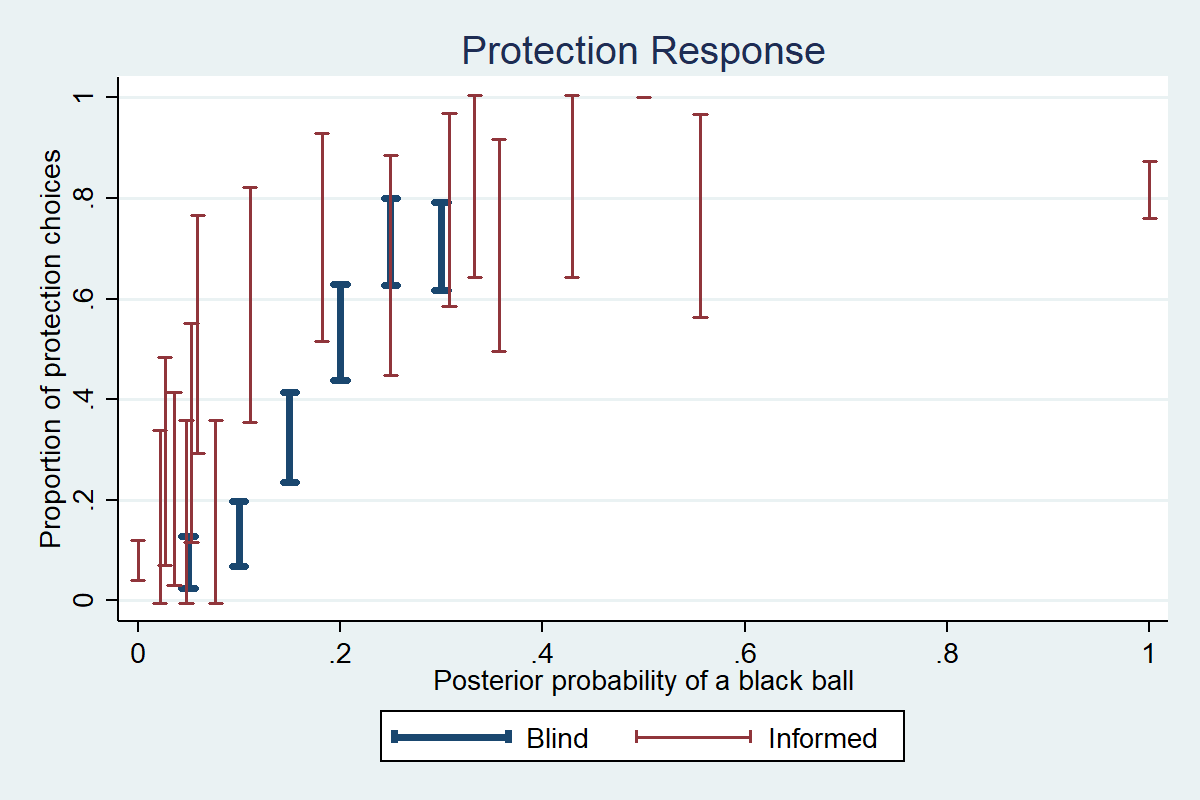
\includegraphics[scale=0.3]{Graphs/ip_response_comp.png}

\end{figure}


\begin{figure}[H]
\centering
\caption{Average Informed Protection Response (Smoothed)} \label{Informed Protection Responses}

  \centering
  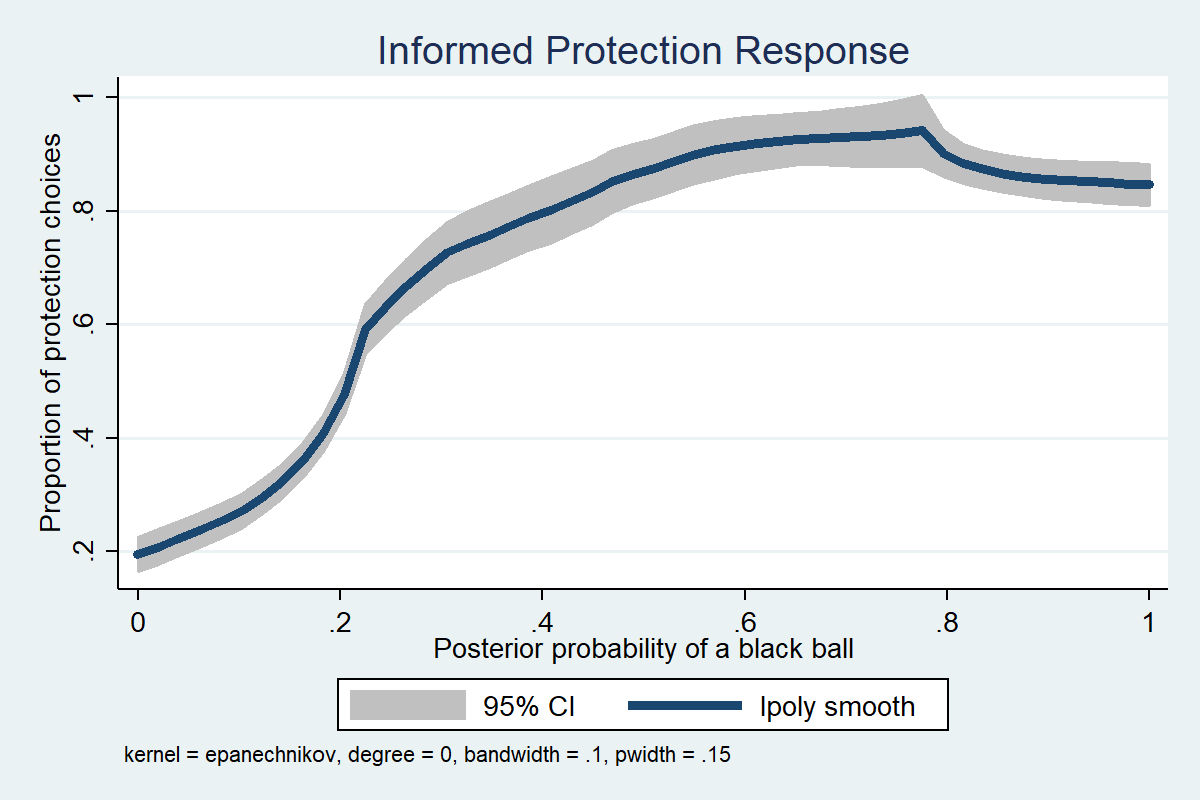
\includegraphics[scale=0.3]{Graphs/ip_response_lpoly.png}

\end{figure}

\begin{figure}[H]
\centering
\caption{Belief Updating}
\begin{subfigure}[t]{.48\textwidth}
  \centering
  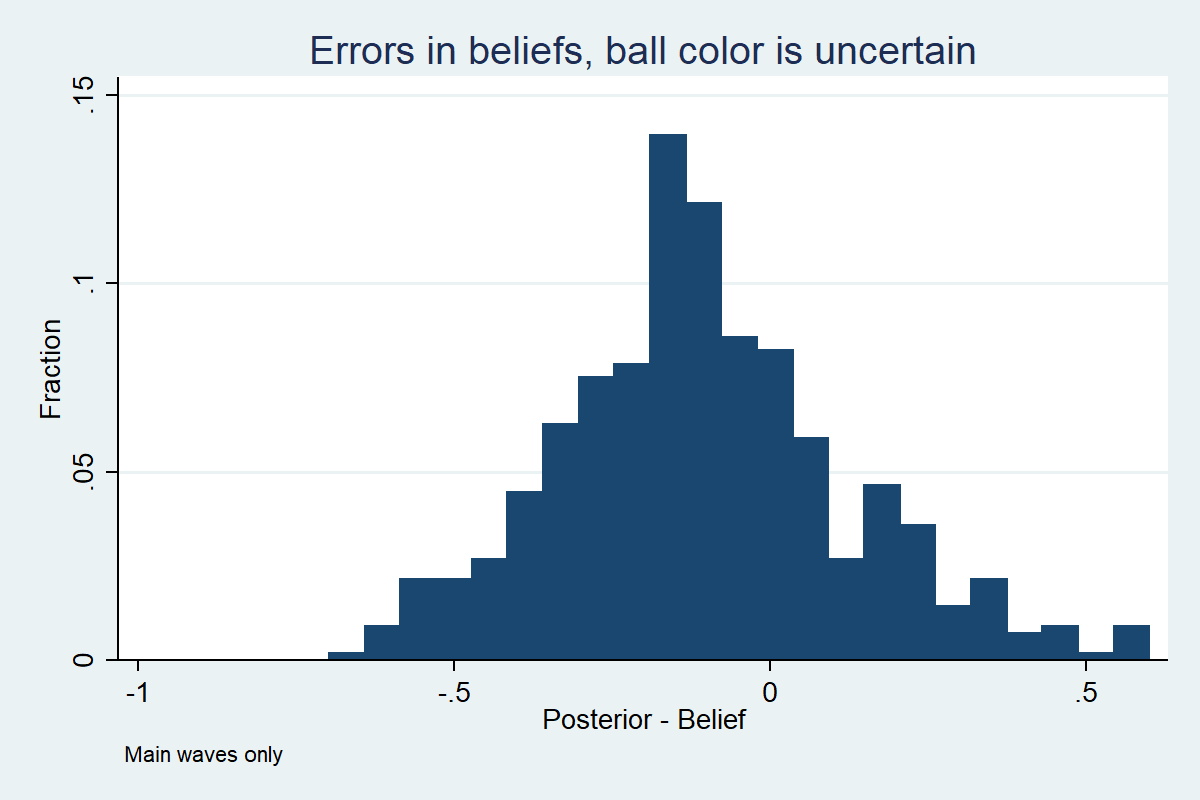
\includegraphics[width=\textwidth]{Graphs/hist_belief_error_s4.png}
\end{subfigure}
\begin{subfigure}[t]{.48\textwidth}
  \centering
  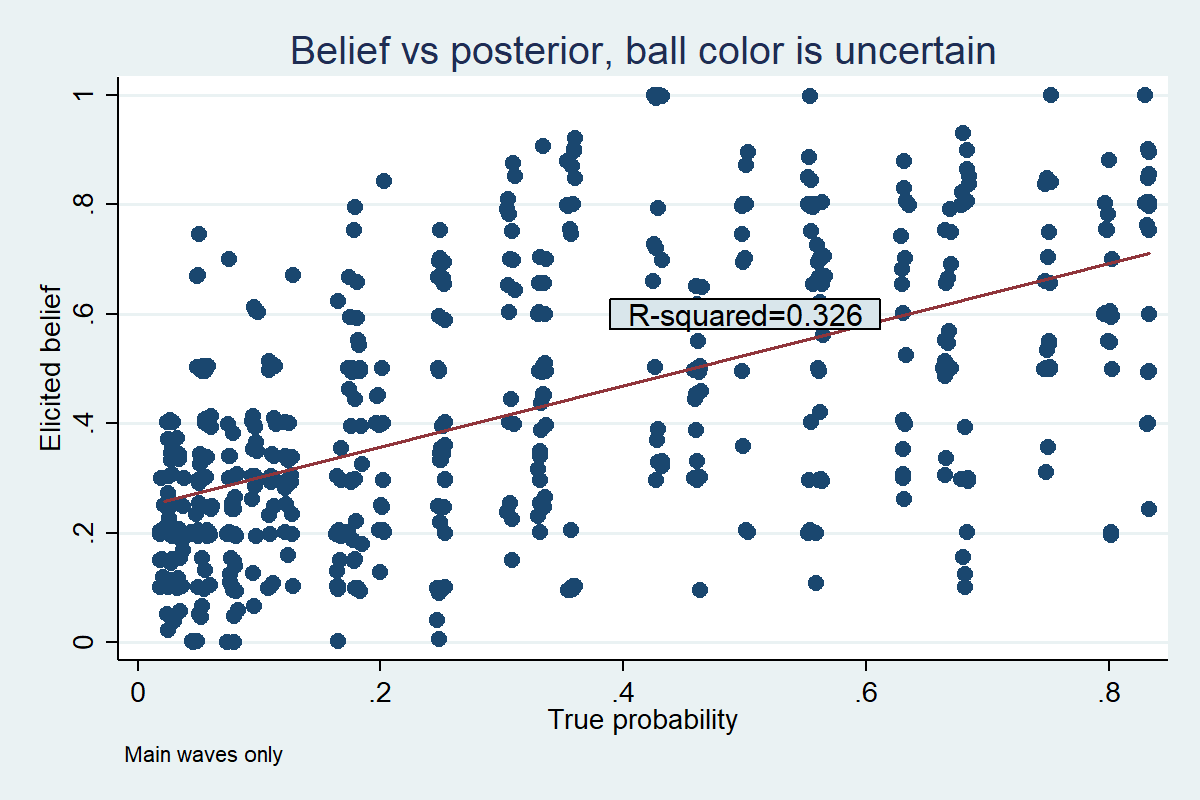
\includegraphics[width=\textwidth]{Graphs/updating_s4.png}

\end{subfigure}
\begin{subfigure}[t]{.48\textwidth}
  \centering
  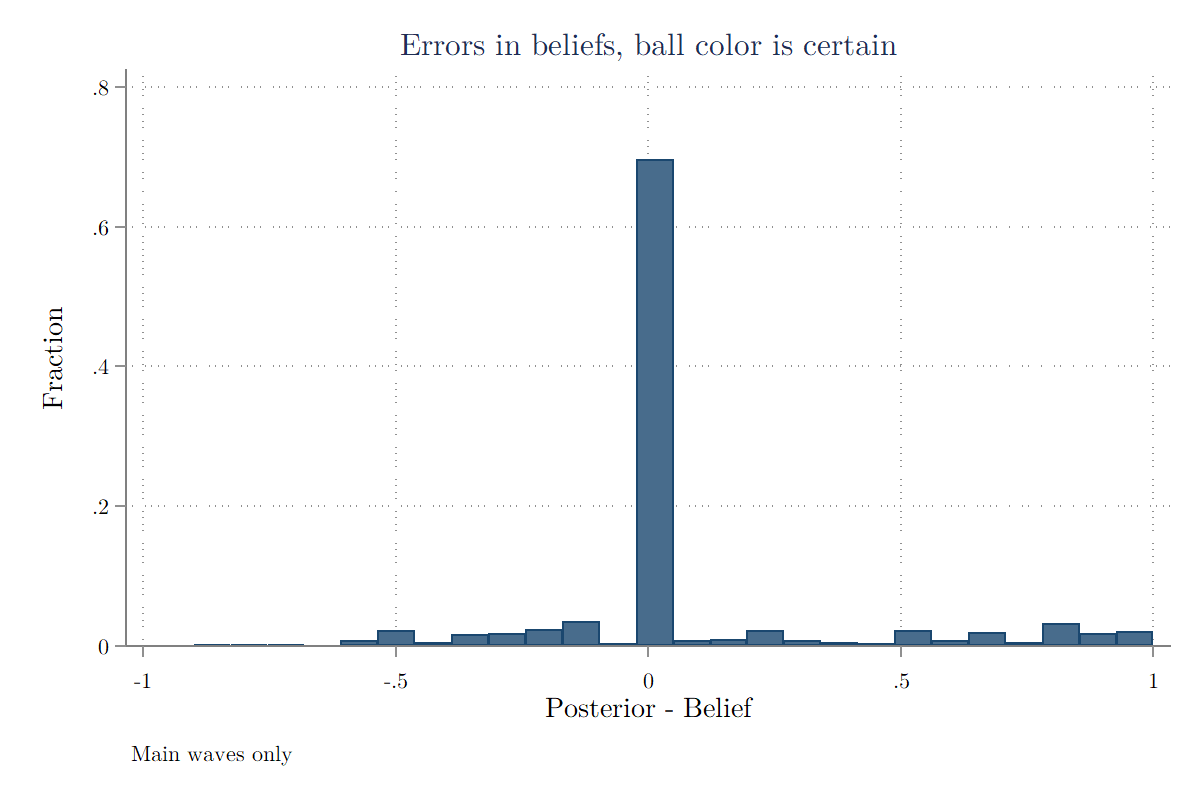
\includegraphics[width=\textwidth]{Graphs/hist_belief_error_s5.png}
\end{subfigure}
\begin{subfigure}[t]{.48\textwidth}
  \centering
  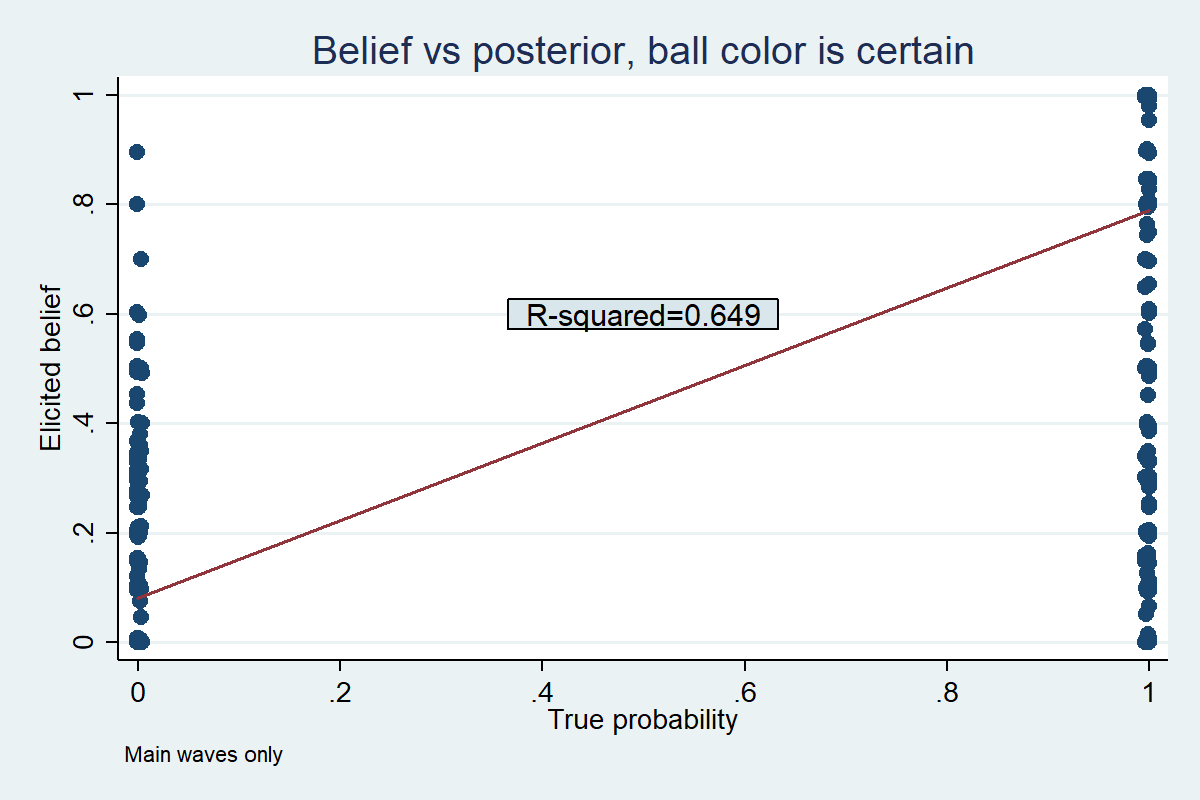
\includegraphics[width=\textwidth]{Graphs/updating_s5.png}

\end{subfigure}

\end{figure}

\begin{figure}[H]
\centering
\caption{Theoretical vs actual WTP}
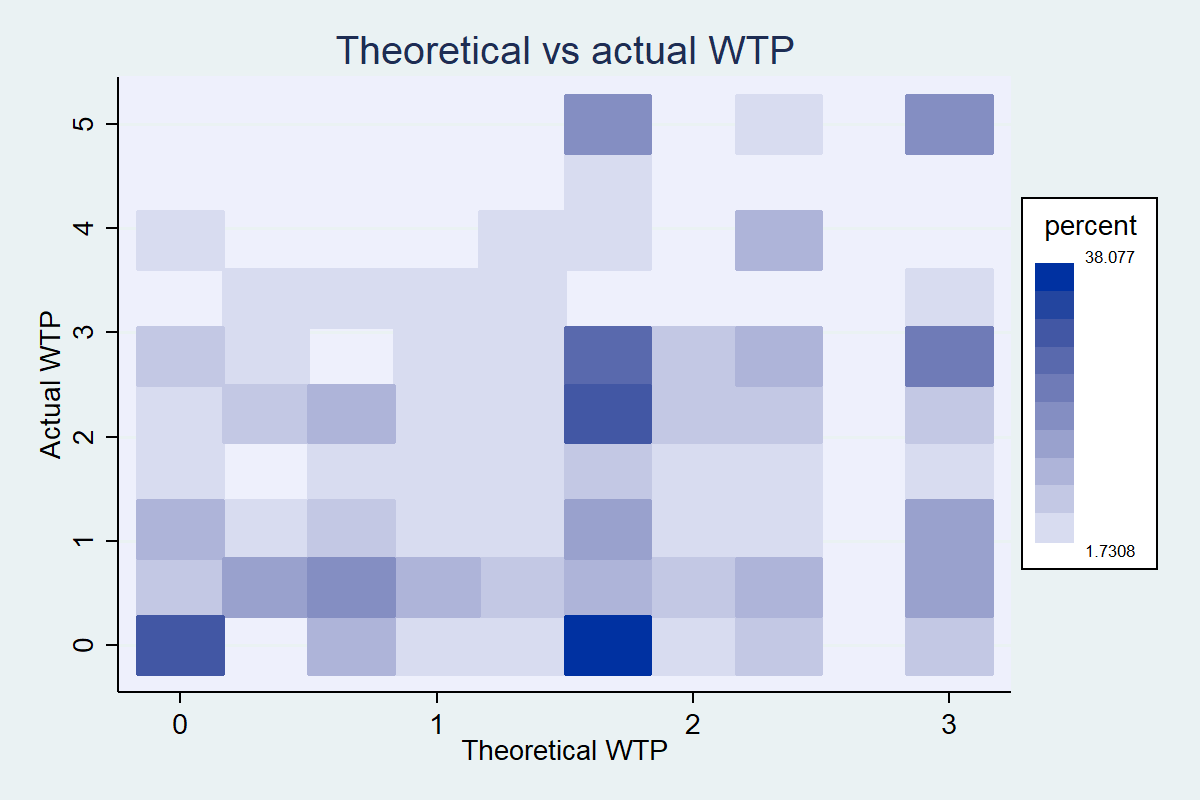
\includegraphics[width=\textwidth]{Graphs/WTP_value_heat.png}
\end{figure}

\begin{figure}[H]
\centering
\caption{WTP discrepancy} \label{WTP_discrepancy}

  \centering
  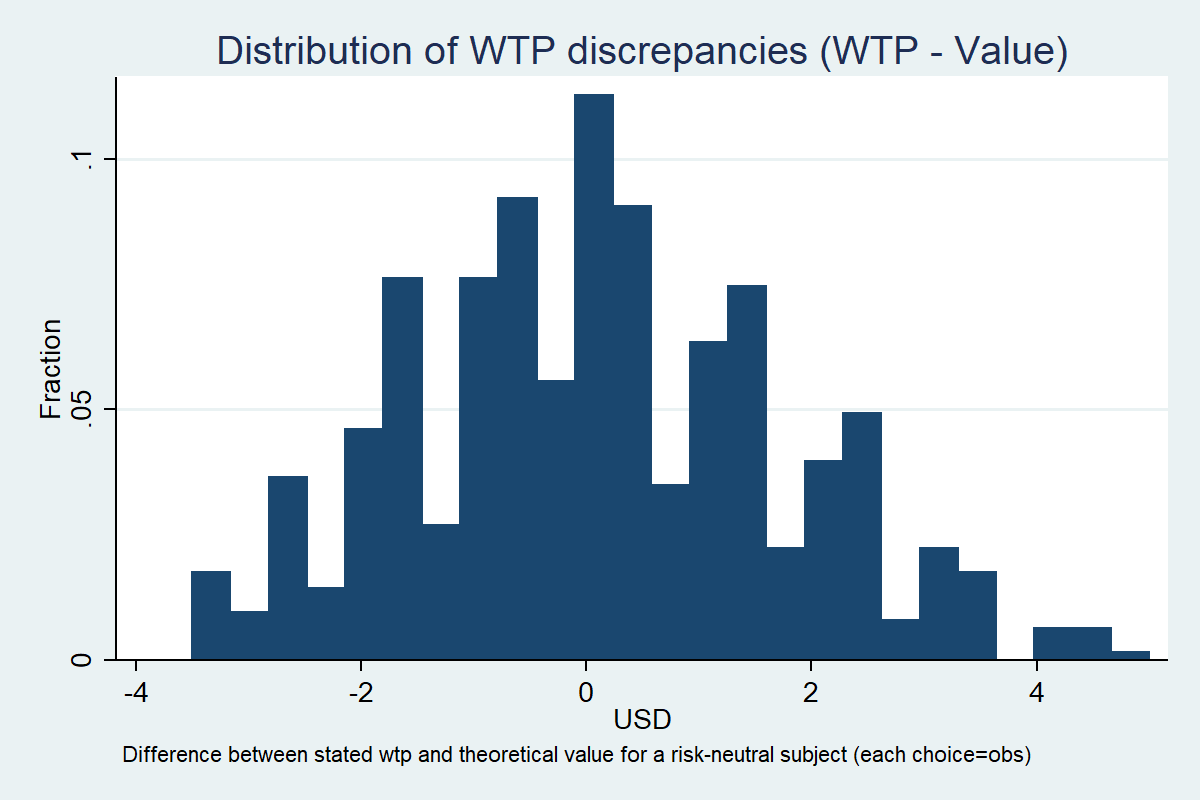
\includegraphics[scale=0.3]{Graphs/hist_WTP_discr1.png}

\end{figure}



\begin{figure}[H]
\caption{WTP discrepancy by prior and signal characteristics} \label{WTP_discr_heat}
\begin{subfigure}{0.5\textwidth}
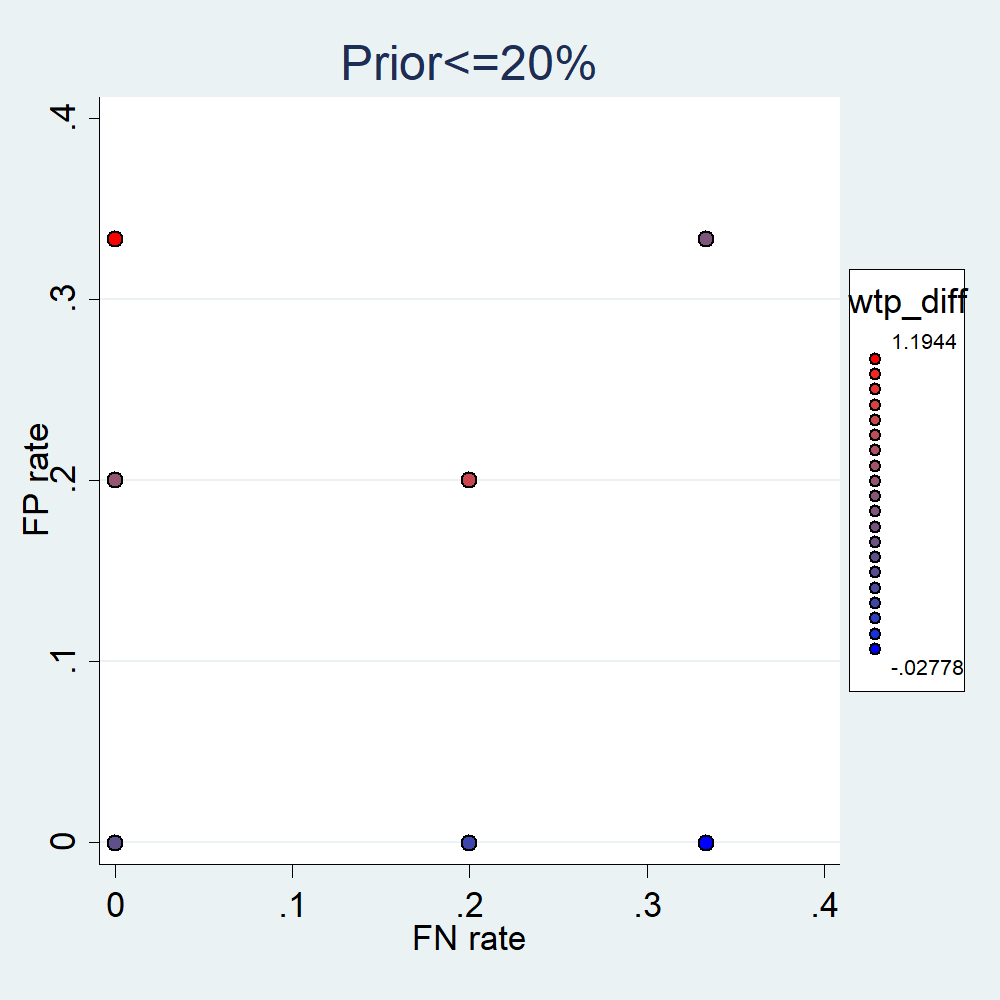
\includegraphics[width=\textwidth]{Graphs/WTP_pattern_low.png}
\end{subfigure}
~
\begin{subfigure}{0.5\textwidth}
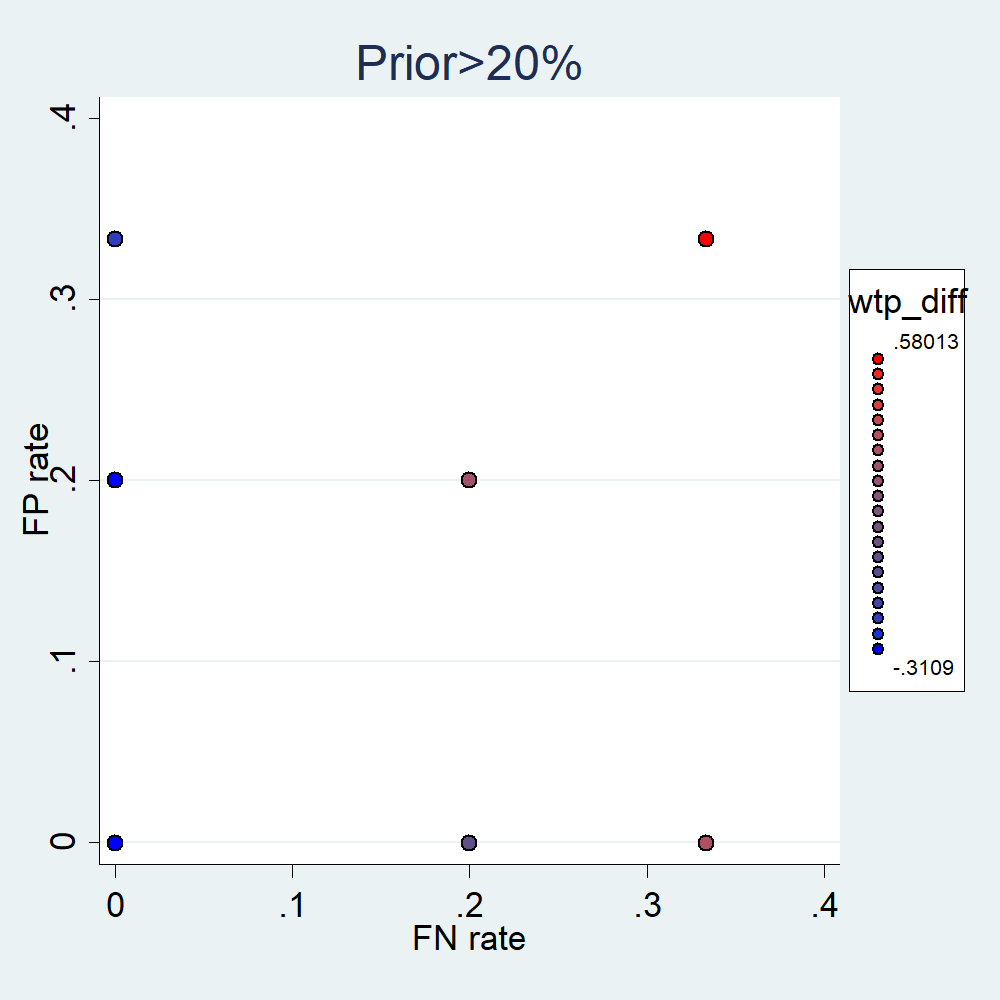
\includegraphics[width=\textwidth]{Graphs/WTP_pattern_high.png}
\end{subfigure}
\end{figure}



\newpage
\section{Appendix Tables}
\begin{table}[htbp]\centering
\def\sym#1{\ifmmode^{#1}\else\(^{#1}\)\fi}
\caption{Informed protection response: linear regression}
\begin{tabular}{l*{6}{c}}
\hline\hline
                &\multicolumn{1}{c}{(1)}&\multicolumn{1}{c}{(2)}&\multicolumn{1}{c}{(3)}&\multicolumn{1}{c}{(4)}&\multicolumn{1}{c}{(5)}&\multicolumn{1}{c}{(6)}\\
                &\multicolumn{1}{c}{All}&\multicolumn{1}{c}{S=White}&\multicolumn{1}{c}{S=Black}&\multicolumn{1}{c}{All}&\multicolumn{1}{c}{S=White}&\multicolumn{1}{c}{W=Black}\\
\hline
FP rate         &     .276\sym{***}&     .524\sym{***}&    .0274         &     .284\sym{***}&     .496\sym{***}&    .0725         \\
                &    (3.0)         &    (4.0)         &    (0.2)         &    (2.9)         &    (3.8)         &    (0.5)         \\
FN rate         &     .616\sym{***}&     1.23\sym{***}&   .00395         &     .596\sym{***}&     1.21\sym{***}&   -.0213         \\
                &    (7.6)         &    (9.7)         &    (0.0)         &    (7.2)         &    (8.9)         &   (-0.2)         \\
plevel=200      &     .106\sym{***}&    .0911\sym{*}  &     .121\sym{**} &     .382\sym{***}&     .693\sym{***}&    .0718\sym{***}\\
                &    (2.8)         &    (1.9)         &    (2.2)         &   (22.5)         &   (27.9)         &    (2.8)         \\
plevel=300      &     .167\sym{***}&     .164\sym{***}&      .17\sym{***}&     .167\sym{***}&     .164\sym{***}&      .17\sym{***}\\
                &    (6.7)         &    (6.2)         &    (4.0)         &    (6.4)         &    (5.7)         &    (3.6)         \\
plevel=500      &     .174\sym{***}&     .202\sym{***}&     .147\sym{***}&     .451\sym{***}&     .804\sym{***}&     .098\sym{***}\\
                &    (4.5)         &    (4.1)         &    (2.7)         &   (26.6)         &   (32.4)         &    (3.9)         \\
Constant        &     .334\sym{***}&   -.0699\sym{**} &     .738\sym{***}&     .402\sym{***}&     -.11\sym{***}&     .913\sym{***}\\
                &   (10.8)         &   (-2.2)         &   (14.4)         &   (22.5)         &   (-4.7)         &   (31.6)         \\
Subject FE      &       No         &       No         &       No         &      Yes         &      Yes         &      Yes         \\
\hline
Observations    &     1248         &      624         &      624         &     1248         &      624         &      624         \\
Adjusted \(R^{2}\)&     0.06         &     0.23         &     0.03         &     0.08         &     0.41         &     0.28         \\
\hline\hline
\multicolumn{7}{l}{\footnotesize \textit{t} statistics in parentheses}\\
\multicolumn{7}{l}{\footnotesize Errors are clustered by subject}\\
\multicolumn{7}{l}{\footnotesize \sym{*} \(p<0.10\), \sym{**} \(p<0.05\), \sym{***} \(p<0.01\)}\\
\end{tabular}
\end{table}

\begin{table}[htbp]\centering
\def\sym#1{\ifmmode^{#1}\else\(^{#1}\)\fi}
\caption{Informed Protection Response: flexible control for posteriors and beliefs}
\begin{tabular}{l*{6}{c}}
\hline\hline
                &\multicolumn{1}{c}{(1)}&\multicolumn{1}{c}{(2)}&\multicolumn{1}{c}{(3)}&\multicolumn{1}{c}{(4)}&\multicolumn{1}{c}{(5)}&\multicolumn{1}{c}{(6)}\\
                &\multicolumn{1}{c}{}&\multicolumn{1}{c}{FE}&\multicolumn{1}{c}{}&\multicolumn{1}{c}{}&\multicolumn{1}{c}{S=White}&\multicolumn{1}{c}{S=Black}\\
\hline
FP rate         &     .323\sym{**} &      .29         &      .29         &     .379\sym{*}  &      .34\sym{***}&    .0312         \\
                &    (2.3)         &    (1.5)         &    (1.3)         &    (1.9)         &    (2.7)         &    (0.1)         \\
FN rate         &    .0616         &    .0446         &   -.0252         &     .583         &   -.0967         &    .0495         \\
                &    (0.5)         &    (0.3)         &   (-0.1)         &    (1.2)         &   (-0.3)         &    (0.3)         \\
p$\geq$0.2      &                  &                  &      .29\sym{***}&                  &                  &                  \\
                &                  &                  &    (4.7)         &                  &                  &                  \\
FP rate x (p $\geq$ 0.2)&                  &                  &    .0154         &                  &                  &                  \\
                &                  &                  &    (0.1)         &                  &                  &                  \\
FN rate x (p $\geq$ 0.2)&                  &                  &     .141         &                  &                  &                  \\
                &                  &                  &    (0.7)         &                  &                  &                  \\
S=Black         &                  &                  &                  &     .706         &                  &                  \\
                &                  &                  &                  &    (1.3)         &                  &                  \\
FP rate x (S=Black)&                  &                  &                  &    -.887         &                  &                  \\
                &                  &                  &                  &   (-1.2)         &                  &                  \\
FN rate x (S=Black)&                  &                  &                  &    -.638         &                  &                  \\
                &                  &                  &                  &   (-1.2)         &                  &                  \\
\hline
Observations    &      624         &      582         &      582         &      582         &      310         &      312         \\
Adjusted \(R^{2}\)&                  &                  &                  &                  &                  &                  \\
\hline\hline
\multicolumn{7}{l}{\footnotesize \textit{t} statistics in parentheses}\\
\multicolumn{7}{l}{\footnotesize With flexible controls of posterior probability and beliefs}\\
\multicolumn{7}{l}{\footnotesize Errors are clustered by subject, average marginal treatment effects}\\
\multicolumn{7}{l}{\footnotesize \sym{*} \(p<0.10\), \sym{**} \(p<0.05\), \sym{***} \(p<0.01\)}\\
\end{tabular}
\end{table}

\begin{table}[htbp]\centering
\def\sym#1{\ifmmode^{#1}\else\(^{#1}\)\fi}
\caption{Informed protection response: semiparametric control for posteriors}
\begin{tabular}{l*{4}{c}}
\hline\hline
                &\multicolumn{1}{c}{(1)}&\multicolumn{1}{c}{(2)}&\multicolumn{1}{c}{(3)}&\multicolumn{1}{c}{(4)}\\
                &\multicolumn{1}{c}{}&\multicolumn{1}{c}{}&\multicolumn{1}{c}{}&\multicolumn{1}{c}{}\\
\hline
FP rate         &     .414\sym{***}&     .463\sym{***}&     .449\sym{***}&     .322\sym{**} \\
                &    (4.2)         &    (2.8)         &    (4.2)         &    (2.4)         \\
FN rate         &    .0152         &   -.0509         &   -.0771         &    .0573         \\
                &    (0.1)         &   (-0.3)         &   (-0.3)         &    (0.4)         \\
p$=$0.2         &                  &    .0471         &                  &                  \\
                &                  &    (1.3)         &                  &                  \\
FP rate x (p $\geq$ 0.2)&                  &   -.0368         &                  &                  \\
                &                  &   (-0.2)         &                  &                  \\
FN rate x (p $\geq$ 0.2)&                  &    .0969         &                  &                  \\
                &                  &    (0.5)         &                  &                  \\
S=Black         &                  &                  &    .0801         &                  \\
                &                  &                  &    (0.5)         &                  \\
FP rate x (S=Black)&                  &                  &     -.41         &                  \\
                &                  &                  &   (-1.0)         &                  \\
FN rate x (S=Black)&                  &                  &      .12         &                  \\
                &                  &                  &    (0.5)         &                  \\
Stat. class     &                  &                  &                  &   -.0101         \\
                &                  &                  &                  &   (-0.3)         \\
FP rate x Stat. class&                  &                  &                  &     .163         \\
                &                  &                  &                  &    (1.1)         \\
FN rate x Stat. class&                  &                  &                  &   -.0696         \\
                &                  &                  &                  &   (-0.5)         \\
\hline
Observations    &     1248         &     1248         &     1248         &     1248         \\
Adjusted \(R^{2}\)&     0.01         &     0.01         &     0.01         &     0.01         \\
\hline\hline
\multicolumn{5}{l}{\footnotesize \textit{t} statistics in parentheses}\\
\multicolumn{5}{l}{\footnotesize \sym{*} \(p<0.10\), \sym{**} \(p<0.05\), \sym{***} \(p<0.01\)}\\
\end{tabular}
\end{table}


\begin{table}[htbp]\centering
\def\sym#1{\ifmmode^{#1}\else\(^{#1}\)\fi}
\caption{WTP - Value of Information, by prior with order effects}
\begin{tabular}{l*{6}{c}}
\hline\hline
                &\multicolumn{1}{c}{(1)}&\multicolumn{1}{c}{(2)}&\multicolumn{1}{c}{(3)}&\multicolumn{1}{c}{(4)}&\multicolumn{1}{c}{(5)}&\multicolumn{1}{c}{(6)}\\
                &\multicolumn{1}{c}{p=0.1,0.2}&\multicolumn{1}{c}{p=0.3,0.5}&\multicolumn{1}{c}{p=0.1,0.2}&\multicolumn{1}{c}{}&\multicolumn{1}{c}{}&\multicolumn{1}{c}{}\\
\hline
FP rate         &     2.23\sym{***}&    -.249         &     2.12\sym{***}&     1.21\sym{*}  &    -.249         &    -.325         \\
                &    (0.5)         &    (0.7)         &    (0.7)         &    (0.7)         &    (0.7)         &    (0.8)         \\
FN rate         &    -.254         &     2.64\sym{***}&    -1.22\sym{**} &     .169         &     2.64\sym{***}&     1.33\sym{***}\\
                &    (0.4)         &    (0.5)         &    (0.5)         &    (0.5)         &    (0.5)         &    (0.5)         \\
Starts with p=0.2&                  &                  &    -1.13\sym{***}&     .256         &                  &                  \\
                &                  &                  &    (0.3)         &    (0.3)         &                  &                  \\
Starts with p=0.2 $\times$ FP rate&                  &                  &     .215         &    -.444         &                  &     .157         \\
                &                  &                  &    (1.0)         &    (1.0)         &                  &    (0.7)         \\
Starts with p=0.2 $\times$ FN rate&                  &                  &     1.99\sym{***}&     2.11\sym{***}&                  &     2.71\sym{***}\\
                &                  &                  &    (0.7)         &    (0.8)         &                  &    (0.6)         \\
First prior     &                  &                  &                  &                  &    .0367         &    .0367         \\
                &                  &                  &                  &                  &    (0.2)         &    (0.2)         \\
First prior $\times$ FP rate&                  &                  &                  &                  &     2.48\sym{***}&     2.48\sym{***}\\
                &                  &                  &                  &                  &    (0.7)         &    (0.7)         \\
First prior $\times$ FN rate&                  &                  &                  &                  &     -2.9\sym{***}&     -2.9\sym{***}\\
                &                  &                  &                  &                  &    (0.3)         &    (0.3)         \\
Constant        &    -.135         &    -.172         &     .412\sym{*}  &    -.278         &    -.172         &    -.172         \\
                &    (0.2)         &    (0.2)         &    (0.2)         &    (0.2)         &    (0.2)         &    (0.2)         \\
\hline
Observations    &      315         &      315         &      315         &      630         &      630         &      630         \\
Adjusted \(R^{2}\)&     0.04         &     0.04         &     0.12         &     0.04         &     0.04         &     0.06         \\
\hline\hline
\multicolumn{7}{l}{\footnotesize Standard errors in parentheses}\\
\multicolumn{7}{l}{\footnotesize \sym{*} \(p<0.10\), \sym{**} \(p<0.05\), \sym{***} \(p<0.01\)}\\
\end{tabular}
\end{table}


\begin{table}[htbp]\centering
\def\sym#1{\ifmmode^{#1}\else\(^{#1}\)\fi}
\caption{WTP for Information (Discrepancy, by prior)}
\begin{tabular}{l*{4}{c}}
\hline\hline
                &\multicolumn{1}{c}{(1)}&\multicolumn{1}{c}{(2)}&\multicolumn{1}{c}{(3)}&\multicolumn{1}{c}{(4)}\\
                &\multicolumn{1}{c}{0.1}&\multicolumn{1}{c}{0.2}&\multicolumn{1}{c}{0.3}&\multicolumn{1}{c}{0.5}\\
\hline
FP rate         &     2.12\sym{***}&     2.34\sym{***}&     .287         &    -.816         \\
                &    (0.7)         &    (0.7)         &    (0.8)         &    (0.9)         \\
FN rate         &    -1.22\sym{**} &     .768         &     1.56\sym{**} &     3.79\sym{***}\\
                &    (0.5)         &    (0.5)         &    (0.6)         &    (0.7)         \\
Constant        &     .412\sym{*}  &    -.715\sym{***}&    -.968\sym{***}&     .671\sym{**} \\
                &    (0.2)         &    (0.2)         &    (0.2)         &    (0.3)         \\
\hline
Observations    &      162         &      153         &      162         &      153         \\
Adjusted \(R^{2}\)&     0.04         &     0.05         &     0.01         &     0.09         \\
\hline\hline
\multicolumn{5}{l}{\footnotesize Standard errors in parentheses}\\
\multicolumn{5}{l}{\footnotesize \sym{*} \(p<0.10\), \sym{**} \(p<0.05\), \sym{***} \(p<0.01\)}\\
\end{tabular}
\end{table}


\begin{table}[htbp]\centering
\def\sym#1{\ifmmode^{#1}\else\(^{#1}\)\fi}
\caption{Belief Elicitation: Discrepancy}
\begin{tabular}{l*{6}{c}}
\hline\hline
                &\multicolumn{1}{c}{(1)}&\multicolumn{1}{c}{(2)}&\multicolumn{1}{c}{(3)}&\multicolumn{1}{c}{(4)}&\multicolumn{1}{c}{(5)}&\multicolumn{1}{c}{(6)}\\
                &\multicolumn{1}{c}{}&\multicolumn{1}{c}{}&\multicolumn{1}{c}{}&\multicolumn{1}{c}{}&\multicolumn{1}{c}{}&\multicolumn{1}{c}{}\\
\hline
FN rate         &     .016         &     .016         &    -.014         &    -.014         &   -.0562         &   -.0554         \\
                &    (0.1)         &    (0.1)         &    (0.1)         &    (0.1)         &    (0.1)         &    (0.1)         \\
FP rate         &     .919\sym{***}&     .919\sym{***}&     1.07\sym{***}&     1.07\sym{***}&     1.05\sym{***}&     1.05\sym{***}\\
                &    (0.1)         &    (0.1)         &    (0.1)         &    (0.1)         &    (0.1)         &    (0.1)         \\
Good quiz       &                  &                  &    .0469         &    .0673         &                  &                  \\
                &                  &                  &    (0.0)         &    (0.0)         &                  &                  \\
Good quiz $\times$ FN rate&                  &                  &    .0463         &    .0464         &                  &                  \\
                &                  &                  &    (0.1)         &    (0.1)         &                  &                  \\
Good quiz $\times$ FP rate&                  &                  &    -.286\sym{*}  &    -.284\sym{*}  &                  &                  \\
                &                  &                  &    (0.2)         &    (0.2)         &                  &                  \\
Stat. class     &                  &                  &                  &                  &  -.00193         &   -.0127         \\
                &                  &                  &                  &                  &    (0.0)         &    (0.0)         \\
Stat. class $\times$ FN rate&                  &                  &                  &                  &     .127         &     .126         \\
                &                  &                  &                  &                  &    (0.1)         &    (0.1)         \\
Stat. class $\times$ FP rate&                  &                  &                  &                  &    -.229         &    -.226         \\
                &                  &                  &                  &                  &    (0.2)         &    (0.2)         \\
Constant        &    -.076\sym{***}&   -.0656\sym{***}&    -.101\sym{***}&    -.102\sym{***}&   -.0751\sym{***}&   -.0563         \\
                &    (0.0)         &    (0.0)         &    (0.0)         &    (0.0)         &    (0.0)         &    (0.0)         \\
Prior prob dummies &       No         &      Yes         &       No         &      Yes         &       No         &      Yes         \\
\hline
Observations    &      630         &      630         &      630         &      630         &      630         &      630         \\
Adjusted \(R^{2}\)&     0.17         &     0.17         &     0.17         &     0.17         &     0.17         &     0.17         \\
\hline\hline
\multicolumn{7}{l}{\footnotesize Standard errors in parentheses}\\
\multicolumn{7}{l}{\footnotesize \sym{*} \(p<0.10\), \sym{**} \(p<0.05\), \sym{***} \(p<0.01\)}\\
\end{tabular}
\end{table}

\footnotesize
\begin{table}[htbp]\centering
\def\sym#1{\ifmmode^{#1}\else\(^{#1}\)\fi}
\caption{WTP minus Value of Information: demographic determinants}
\begin{tabular}{l*{9}{c}}
\hline\hline
                &\multicolumn{1}{c}{(1)}&\multicolumn{1}{c}{(2)}&\multicolumn{1}{c}{(3)}&\multicolumn{1}{c}{(4)}&\multicolumn{1}{c}{(5)}&\multicolumn{1}{c}{(6)}&\multicolumn{1}{c}{(7)}&\multicolumn{1}{c}{(8)}&\multicolumn{1}{c}{(9)}\\
                &\multicolumn{1}{c}{}&\multicolumn{1}{c}{}&\multicolumn{1}{c}{}&\multicolumn{1}{c}{}&\multicolumn{1}{c}{}&\multicolumn{1}{c}{}&\multicolumn{1}{c}{}&\multicolumn{1}{c}{}&\multicolumn{1}{c}{}\\
\hline
FP costs        &     .558\sym{***}&     .602\sym{***}&     .548\sym{***}&     .475\sym{**} &     .416\sym{**} &      .54\sym{***}&     .485\sym{***}&      .66\sym{***}&     .591\sym{***}\\
                &    (0.1)         &    (0.2)         &    (0.2)         &    (0.2)         &    (0.2)         &    (0.1)         &    (0.1)         &    (0.2)         &    (0.2)         \\
FN costs        &    -.229\sym{*}  &    -.317\sym{*}  &   -.0684         &    -.242         &   -.0701         &    -.295\sym{*}  &   -.0336         &    -.037         &     .223         \\
                &    (0.1)         &    (0.2)         &    (0.2)         &    (0.2)         &    (0.2)         &    (0.2)         &    (0.1)         &    (0.2)         &    (0.2)         \\
Male            &                  &    -.195         &    -.197         &                  &                  &                  &                  &                  &                  \\
                &                  &    (0.4)         &    (0.4)         &                  &                  &                  &                  &                  &                  \\
Male $\times$ FP costs&                  &    -.138         &    -.155         &                  &                  &                  &                  &                  &                  \\
                &                  &    (0.2)         &    (0.2)         &                  &                  &                  &                  &                  &                  \\
Male $\times$ FN costs&                  &     .225         &     .249         &                  &                  &                  &                  &                  &                  \\
                &                  &    (0.3)         &    (0.2)         &                  &                  &                  &                  &                  &                  \\
Stat. class     &                  &                  &                  &    -.161         &    -.179         &                  &                  &                  &                  \\
                &                  &                  &                  &    (0.4)         &    (0.4)         &                  &                  &                  &                  \\
Stat. class $\times$ FP costs&                  &                  &                  &     .138         &     .125         &                  &                  &                  &                  \\
                &                  &                  &                  &    (0.2)         &    (0.2)         &                  &                  &                  &                  \\
Stat. class $\times$ FN costs&                  &                  &                  &    .0192         &     .199         &                  &                  &                  &                  \\
                &                  &                  &                  &    (0.3)         &    (0.2)         &                  &                  &                  &                  \\
$>$23 yrs       &                  &                  &                  &                  &                  &    -.827\sym{**} &    -.785\sym{**} &                  &                  \\
                &                  &                  &                  &                  &                  &    (0.4)         &    (0.3)         &                  &                  \\
$>$23 yrs $\times$ FP costs&                  &                  &                  &                  &                  &     .193         &     .159         &                  &                  \\
                &                  &                  &                  &                  &                  &    (0.3)         &    (0.3)         &                  &                  \\
$>$23 yrs $\times$ FN costs&                  &                  &                  &                  &                  &     .465\sym{**} &     .389         &                  &                  \\
                &                  &                  &                  &                  &                  &    (0.2)         &    (0.3)         &                  &                  \\
Good quiz       &                  &                  &                  &                  &                  &                  &                  &     .347         &     .413         \\
                &                  &                  &                  &                  &                  &                  &                  &    (0.4)         &    (0.4)         \\
Good quiz $\times$ FP costs&                  &                  &                  &                  &                  &                  &                  &    -.194         &    -.178         \\
                &                  &                  &                  &                  &                  &                  &                  &    (0.2)         &    (0.2)         \\
Good quiz $\times$ FN costs&                  &                  &                  &                  &                  &                  &                  &    -.355         &    -.354         \\
                &                  &                  &                  &                  &                  &                  &                  &    (0.3)         &    (0.2)         \\
Constant        &   -.0921         &   -.0115         &     .356         &   .00585         &     .387         &    .0142         &     .363         &    -.279         &    .0568         \\
                &    (0.2)         &    (0.2)         &    (0.3)         &    (0.3)         &    (0.4)         &    (0.2)         &    (0.2)         &    (0.3)         &    (0.3)         \\
Prior dummies   &       No         &       No         &      Yes         &       No         &      Yes         &       No         &      Yes         &       No         &      Yes         \\
\hline
Observations    &      312         &      312         &      312         &      312         &      312         &      312         &      312         &      312         &      312         \\
Adjusted \(R^{2}\)&     0.05         &     0.04         &     0.12         &     0.04         &     0.12         &     0.06         &     0.13         &     0.04         &     0.12         \\
\hline\hline
\multicolumn{10}{l}{\footnotesize Standard errors in parentheses}\\
\multicolumn{10}{l}{\footnotesize \sym{*} \(p<0.10\), \sym{**} \(p<0.05\), \sym{***} \(p<0.01\)}\\
\end{tabular}
\end{table}
 \label{wtp_dem}



\end{document}